\documentclass[11pt,a4paper]{article}
\usepackage{fullpage}
\usepackage{tgadventor}
\usepackage[T1]{fontenc}
\newcommand{\hsp}{\hspace{20pt}}
\newcommand{\HRule}{\rule{\linewidth}{0.5mm}}
\usepackage{float}
\usepackage{amsmath}
\usepackage{caption}
\usepackage{subcaption}
\usepackage{graphicx}
\usepackage{xcolor}
\usepackage{multirow}
\usepackage{hyperref}
\definecolor{darkblue}{RGB}{14,43,88}
\usepackage{chemformula}
\usepackage{verbatim}

\makeatletter
\newcommand{\authors}{%
  \setlength\arrayrulewidth{2pt}
  \begin{tabular}{l|l}
  \@authorsi
}
\newcommand\@authorsi{\@ifnextchar\stopauthors{\@authorsend}{\@authorsii}}
\newcommand\@authorsii[2]{%
  \\
  \textbf{\Large #1} &  \textbf{\Large #2}
  \\
  \@authorsi % restart the recursion
}
\newcommand\@authorsend[1]{
  \end{tabular}}
\makeatother

%%%%%%%%%%%%%%%%%%%%%%%%%%%%%%%%%%%%%%%%%%%%%%%%%%%
%%%%%%%%%%%% Define following Variables %%%%%%%%%%%
%%%%%%%%%%%%%%%%%%%%%%%%%%%%%%%%%%%%%%%%%%%%%%%%%%%
\def \classSigle{LMAPR2451}
\def \className{Atomistic and nanoscopic simulations}
\def \workName{Study of \ch{FeS2} and its optical properties}
\def \professors{Professors Jean-Christophe Charlier, Xavier Gonze \& Gian-Marco Rignanese\\Mentors : Alexandre Cloots \& Ionel-Bogdan Guster}
\def \academicYear{2020-2021}
\def \abstractText{This report aims to investigate the optical properties of \ch{FeS2}. To do so, \textit{ab initio} computations are performed on a 6-atoms orthorhombic unit cell. The convergence with respect to several structural parameters is also studied. The optical properties are then analyzed in the light of the obtained results. Finally, a comparison is made with the published research, and a discussion about the quality of the simulation is made.}
%%%%%%%%%%%%%%%%%%%%%%%%%%%%%%%%%%%%%%%%%%%%%%%%%%%
%%%%%%%%%%%%%%%%%%%%%%%%%%%%%%%%%%%%%%%%%%%%%%%%%%%
%%%%%%%%%%%%%%%%%%%%%%%%%%%%%%%%%%%%%%%%%%%%%%%%%%%

\begin{document}
\begin{titlepage}
\begingroup
\fontfamily{\sfdefault}
  \begin{flushleft}  
  \begin{minipage}{0.55\textwidth}  
\includegraphics[width=\textwidth]{images/epl2.png}
  \end{minipage}
  \end{flushleft}
  \centering
  \textcolor{darkblue}{{\huge \textbf{\classSigle \\[0.1cm] \className}}}
  \vfill
  \textcolor{darkblue}{
  \hrule height 0.1cm
  \hspace{1cm}\\[0.3cm]
  {\Huge \textbf{\workName}}\\[0.5cm]
  \hrule height 0.1cm
  \hspace{1cm}\\[0.3cm]
  {\Large\textbf{\professors}}}
  \vfill
  \begin{minipage}[c]{\textwidth}
  \centering
  \textcolor{darkblue}{
  \authors
  %%%%%%%%%%%%%%%%%%%%%%%%%%%%%%%%%%%%%%%%%%%%%%%%%
  %%%%Mettre un auteur par ligne sous le format%%%%
  %%%%%%%%%%%%%%%%{Nom Prénom}{NOMA}%%%%%%%%%%%%%%%
  %%%%%%%%%%%%%%%%%%%%%%%%%%%%%%%%%%%%%%%%%%%%%%%%%
  {Anatole Moureaux}{54731700}
  %%%%%%%%%%%%%%%%%%%%%%%%%%%%%%%%%%%%%%%%%%%%%%%%%
  %%%%%%%%%%%%%%%%%%%%%%%%%%%%%%%%%%%%%%%%%%%%%%%%%
  %%%%%%%%%%%%%%%%%%%%%%%%%%%%%%%%%%%%%%%%%%%%%%%%%
  \stopauthors}
  \end{minipage}
  \vfill
  \noindent\fbox{%
    \parbox{1\textwidth}{%
        \centering
         \textcolor{darkblue}{\textbf{\abstractText}}%
        }
    }
  \vfill
  \begin{center}
  \textcolor{darkblue}{\textbf{\Large \academicYear}}
  \end{center}
\endgroup
\end{titlepage}
\tableofcontents
\newpage
\section{Introduction}
\subsection{Motivation}
Pyrite (\ch{FeS2}) is an interesting semiconducting material. Indeed, it can be used in numerous domains, from mechanical applications, where it is appreciated for its toughness and abrasiveness, to optical applications, where it can be used as an high-energy light absorber \cite{pyriteApps}. As pyrite is very abundant, it can become a material of choice in the industry if correct and valuable uses of the latter could be elaborated. It is depicted on \autoref{fig:pyriteOre}.

\begin{figure}[H]
\centering
\begin{subfigure}[b]{0.45\textwidth}
\centering
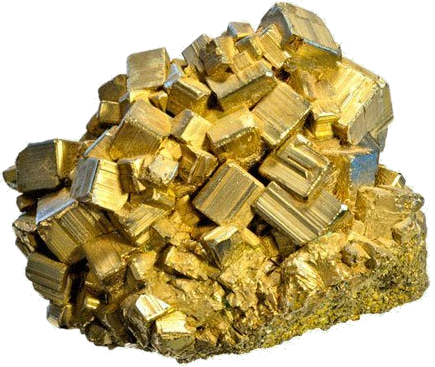
\includegraphics[width=\textwidth]{images/pyrite}
\caption{Pyrite}
\label{fig:pyriteOre}
\end{subfigure}
\hfill
\begin{subfigure}[b]{0.45\textwidth}
\centering
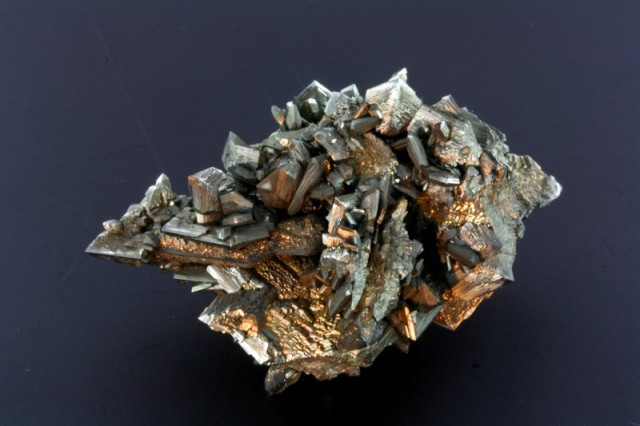
\includegraphics[width=\textwidth]{images/marcassite}
\caption{Marcassite, the orthrhombic polymorph of pyrite}
\label{fig:marcassiteOre}
\end{subfigure}
\caption{\ch{FeS2} ores}
\end{figure}

One of the promising potential application of pyrite is its integration into solar panels. Indeed, pyrite thin films could be good alternatives to the conventional silicon based solar cells, since the latter are more economically and ecologically costly \cite{pyriteSolarCells,Ore}. However, the performances of the material must be similar to or better than materials already used for solar cells, in order to make it truly competitive.

The concept of solar cell dates all the way back to 1883 \cite{solarcellinvention}. However, it is interesting to recall some of the main features of such a device. A solar cell consists of photoelectric components able to convert the energy of the (solar) light into electricity though the \textit{photovoltaic effect}. More precisely, it is composed of a \textit{pn}-junction diode, usually made of silicon. When the depletion region of the junction is hit by solar photons, an electron is delivered in the $n$-layer and a hole is delivered in the $p$-layer (\autoref{fig:pnjunction}). By doing so on a large scale, the \textit{pn}-junction is able to generate a voltage of about $0.5$ V, if the $n$-doped layer is sufficiently thin (to make the photons reach the depletion region as easily as possible). A solar panel is composed of several solar cells in series, in order to add up the voltage generated by each cell. The best materials for solar cells-related applications are the materials showing :
\begin{itemize}
\item a semiconducting behavior
\item a high optical absorption coefficient
\item a high electrical conductivity
\item an abundant presence in the Earth's crust.\cite{solarCell}
\end{itemize}
\begin{figure}[H]
\centering
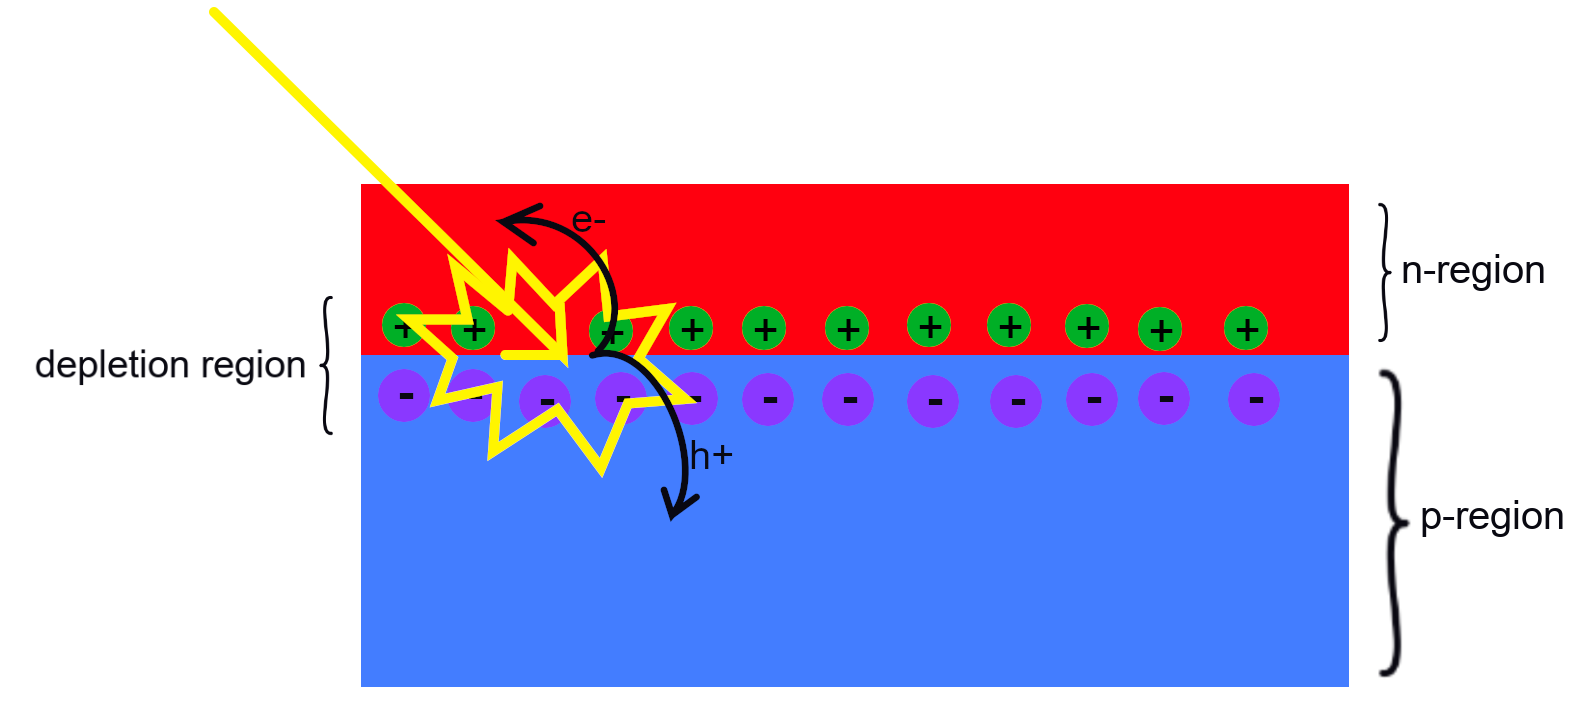
\includegraphics[width=0.8\textwidth]{images/pnjunction.png}
\caption{Simplified view of the photovoltaic effect at the $pn$-junction of a solar cell. The green and purple dots are the charges resulting from the recombination of charge carriers in the depletion region. When a photon hits an atom in the depletion region, an electron is released in the $n$-region and a hole is released in the $p$-region, creating a voltage when repeated multiple times.}
\label{fig:pnjunction}
\end{figure}
Even if bulk pyrite shows a $n$-type behavior, pyrite thin-films show a $p$-type behavior. Only the deposition of a thin layer of $n$-type semiconductor on the pyrite film is needed to form a $pn$-heterojunction. Furthermore, the pyrite has a strong absorption coefficient. It thus allows to decrease the thickness of the pyrite film, which is helpful to improve the performances of the $pn$-junction, and hence, of the solar cell \cite{thinFilms}. Furthermore, it is earth-abundant. Pyrite thus seems to be a material of choice for photovoltaic applications.

However, serious limitations prevent pyrite to be highly performant in this framework. Indeed, a very poor solar energy conversion efficiency is observed when assessing the performances of pyrite solar cells. That low efficiency is presumably due to a low photovoltage generation. The origin of that low photovoltage is highly debated among the scientific community. Several possible sources have been proposed over the years : detrimental \ch{S} vacancies (although stoichimetric pyrite shows the same low photovoltage), detrimental impurities or even lattice defects \cite{limitations}. No consensus has been found so far. But as pyrite could be a game-changer in the solar cell industry if its efficiency were improved, it is worth to look a little closer to the optical properties of the material.

In the following report, the properties of the \ch{FeS2} in the Pnnm space group will be studied using the \texttt{Abinit} package \cite{Abinit}. As the unit cell of pyrite, which contains 12 atoms, is close to the computational limits of \texttt{Abinit}, the computations will be performed on a 6-atoms orthorhombic polymorph, depicted on \autoref{fig:marcassiteOre}. The results will be used as a starting point for the reflection concerning the actual pyrite. First, the unit cell and its structural parameters will be described, based on the Materials Project documentation\footnote{\url{https://materialsproject.org/materials/mp-1522/}}. Then, the representation of the crystal in \texttt{Abinit} will be presented. Secondly, the pseudopotential and the approximation used in the first place will be discussed. Then, the convergence of the total energy per atom and the lattice scale parameters, with respect to the energy cut-off (\texttt{ecut}) and the number of $k$-points (\texttt{ngkpt}) will be studied. After that, \texttt{Abinit} computations will be performed using the converged values and the optical properties will be studied. To conclude, the obtained results will be compared with the published research.
\subsection{\ch{FeS2} : Overview and \texttt{Abinit} representation}
The orthorhombic \ch{FeS2} primitive cell contains 2 Fe atoms and 4 S atoms (\autoref{fig:primitiveCell}). The space group is Pnnm[58] in the Hermann-Mauguin notation. 

Furthermore, it is a semiconductor. The energy of the indirect bandgap is about 0.978 eV\cite{MaterialsProject}.

Finally, the primitive cell will be represented as follow in \texttt{Abinit} input files :
\begin{center}
\begin{tabular}{lll}
\texttt{acell} & \texttt{3.390} \texttt{4.438} \texttt{5.411} \texttt{Angstr} & \texttt{\# the lattice vectors scaling}\\
\texttt{ntypat} & \texttt{2} & \texttt{\# there are two types of atoms in the}\\
&&\texttt{\#\space\space\space\space primitive cell : Fe and S}\\
\texttt{znucl} & \texttt{26 16}& \texttt{\# Fe has 26 electrons and S has 16}\\
\texttt{natom} & \texttt{6} & \texttt{\# there are 6 atoms in the primitive cell}\\
\texttt{typat} & \texttt{1 1 2 2 2 2}&\texttt{\# 2 Fe atoms and 4 S atoms}\\
\texttt{xred} & \texttt{0\space\space\space\space\space\space 0\space\space\space\space\space\space 0} & \texttt{\# position of the first Fe atom in reduced coordinates}\\
& \texttt{0.5\space\space\space\space 0.5\space\space\space\space0.5} & \texttt{\# position of the second Fe atom}\\
& \texttt{0\space\space\space\space\space\space 0.206\space\space 0.3753} & \texttt{\# position of the first S atom}\\
& \texttt{0\space\space\space\space\space\space 0.794\space\space 0.6247} & \texttt{\# position of the second S atom}\\
& \texttt{0.5\space\space\space\space 0.294\space\space 0.8753} & \texttt{\# position of the third S atom}\\
& \texttt{0.5\space\space\space\space 0.706\space\space 0.1247} & \texttt{\# position of the fourth S atom}\\
\end{tabular}
\end{center} 
The data also comes from the Materials Project \cite{MaterialsProject}.
\begin{figure}[H]
\centering
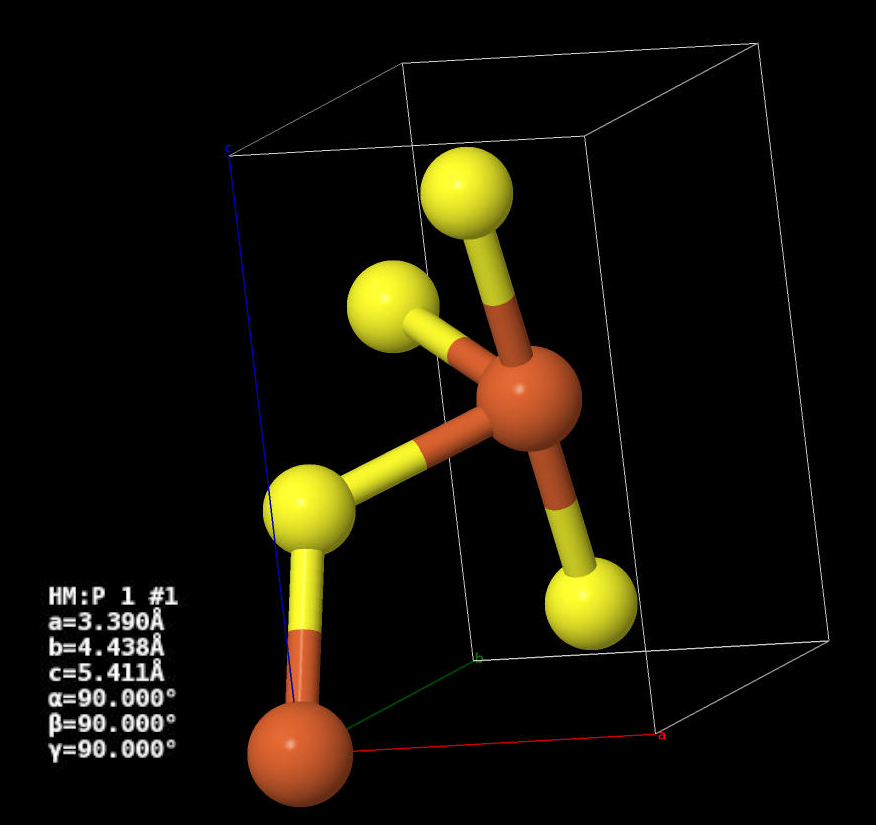
\includegraphics[width=\textwidth]{images/primitiveCell.eps}
\caption{Primitive cell of orthorhombic \ch{FeS2}.\\Materials Project (mp-1522), Vesta}
\label{fig:primitiveCell}
\end{figure}
\newpage
\section{Convergence studies and pseudopotentials}
In DFT computations, convergence studies are very important. They are meant to ensure that the chosen input parameters, like the cut-off energy (\texttt{ecut}) or the number of $k$-points in the cell (determined by the sampling of the Brillouin zone \texttt{ngkpt}), allow accurate results while limiting the computational time as much. To perform such an analysis, the same computations are repeated using datasets with various values of the parameter of interest, with an increasing accuracy of the environment. The evolution of some calculated variables, like the total energy of the unit cell (\texttt{etotal}), indicates when the parameters of interest guarantee a sufficiently accurate simulation.

In the following subsections, the convergence of the total energy per atom and of the lattice scale parameters will be studied with respect to \texttt{ecut} and \texttt{ngkpt}.
\subsection{Additional parameters}
To begin, we will use the \textit{Local Density Approximation} (LDA) functional. The pseudopotentials that will be used are retrieved from the PseudoDojo \cite{PseudoDojo}. Two pseudopotentials are used : the NC SR (ONCVPSP v0.4.1) LDA standard pseudopotential relative to Fe, and the same one but relative to S (both in psp8 format). The pseudopotentials respectively consider 16 electrons ($3s^23p^64s^23d^6$ for \ch{Fe}) and 6 electrons ($3s^23p^4$ for \ch{S}) so that the unit cell contains 56 electrons.

It is also important to properly define the parameters ruling the SCF procedure. The most important one is \texttt{nstep}, defining the number of allowed SCF cycles to reach convergence. It is set to \texttt{100} in the first place. \texttt{toldfe}, the difference of total energy between two SCF cycles defining the moment when convergence is reached, is set to \texttt{1.0d-10} Ha. \texttt{toldfe} is chosen as the structural relaxation is not performed yet (in that case, \texttt{toldff} or \texttt{tolrff} is preferably used). Although it is not mandatory, the SCF procedure can be preconditioned by specifying the macroscopic dielectric constant (\texttt{diemac}). It is used to speed up the SCF procedure. A value of \texttt{24} is chosen, accordingly to the Materials Project \cite{MaterialsProject}. 

Finally, the parameters of the $k$-points grid must be specified. \texttt{kptopt} is set to \texttt{1} in order to take advantage of the symmetry of the unit cell. 
By setting \texttt{prtkpt} to \texttt{1}, \texttt{Abinit} will generate a set of $k$-point grids, that will be helpful to optimize further computations and convergence studies.
\begin{center}
\begin{tabular}{lll}
\texttt{pseudos} & \multicolumn{2}{l}{\texttt{"pdj\_nc\_sr\_041\_lda\_standard\_psp8/Fe.psp8, pdj\_nc\_sr\_041\_lda\_standard\_psp8/S.psp8"}}\\
&&\\
\multicolumn{3}{l}{\texttt{\# parameters of the SCF procedure : }}\\
\texttt{nstep} & \texttt{100} &\texttt{\# maximal number of SCF cycles}\\
\texttt{toldfe} & \texttt{1.0d-10} &\texttt{\# SCF procedure will stop when the difference of total energy}\\
&&\texttt{\#\space\space\space\space between two iterations will be lower than toldfe Hartree}\\
\texttt{diemac} &\texttt{24.0} & \texttt{\# preconditioning of the SCF procedure.}\\
&&\\
\multicolumn{3}{l}{\texttt{\# parameters of the k-points grid : }}\\
\texttt{kptopt} & \texttt{1} &\\
\texttt{prtkpt} & \texttt{1} 
\end{tabular}
\end{center}
\subsection{Convergence of the total energy per atom as a function of the cut-off energy (\texttt{ecut})}
In the next computations, the default Monkhorst-Pack grids will be used. 4 $k$-points will be sampled along the longest lattice direction ([0 0 1]). To keep a constant density of $k$-points along each axis, 3 $k$-points will be sampled along directions [1 0 0] and  [0 1 0]. The input lattice parameters are thus :
\begin{center}
\begin{tabular}{lll}
\texttt{ngkpt} & \texttt{3 3 4}&\\
\texttt{nshiftk} & \texttt{1} &\\
\texttt{shiftk} &\texttt{0.5 0.5 0.5}
\end{tabular}
\end{center}
The study of the convergence of the simulation was performed by running \texttt{Abinit} with the input file \texttt{1522\_3\_ecutConv.abi} (\autoref{Abi1}).
The total energy per atom of the unit cell is then plotted versus \texttt{ecut} (which spans from $10$ [Ha] to $59$ [Ha]) (\autoref{fig:ecutConv}). Upper and lower bounds of $\pm 0.5$ [mHa] are set around the last obtained value. It allows to determine the first \texttt{ecut} for which the convergence is reasonable. In the present case, \texttt{ecut} = \texttt{40} [Ha].
\begin{figure}[H]
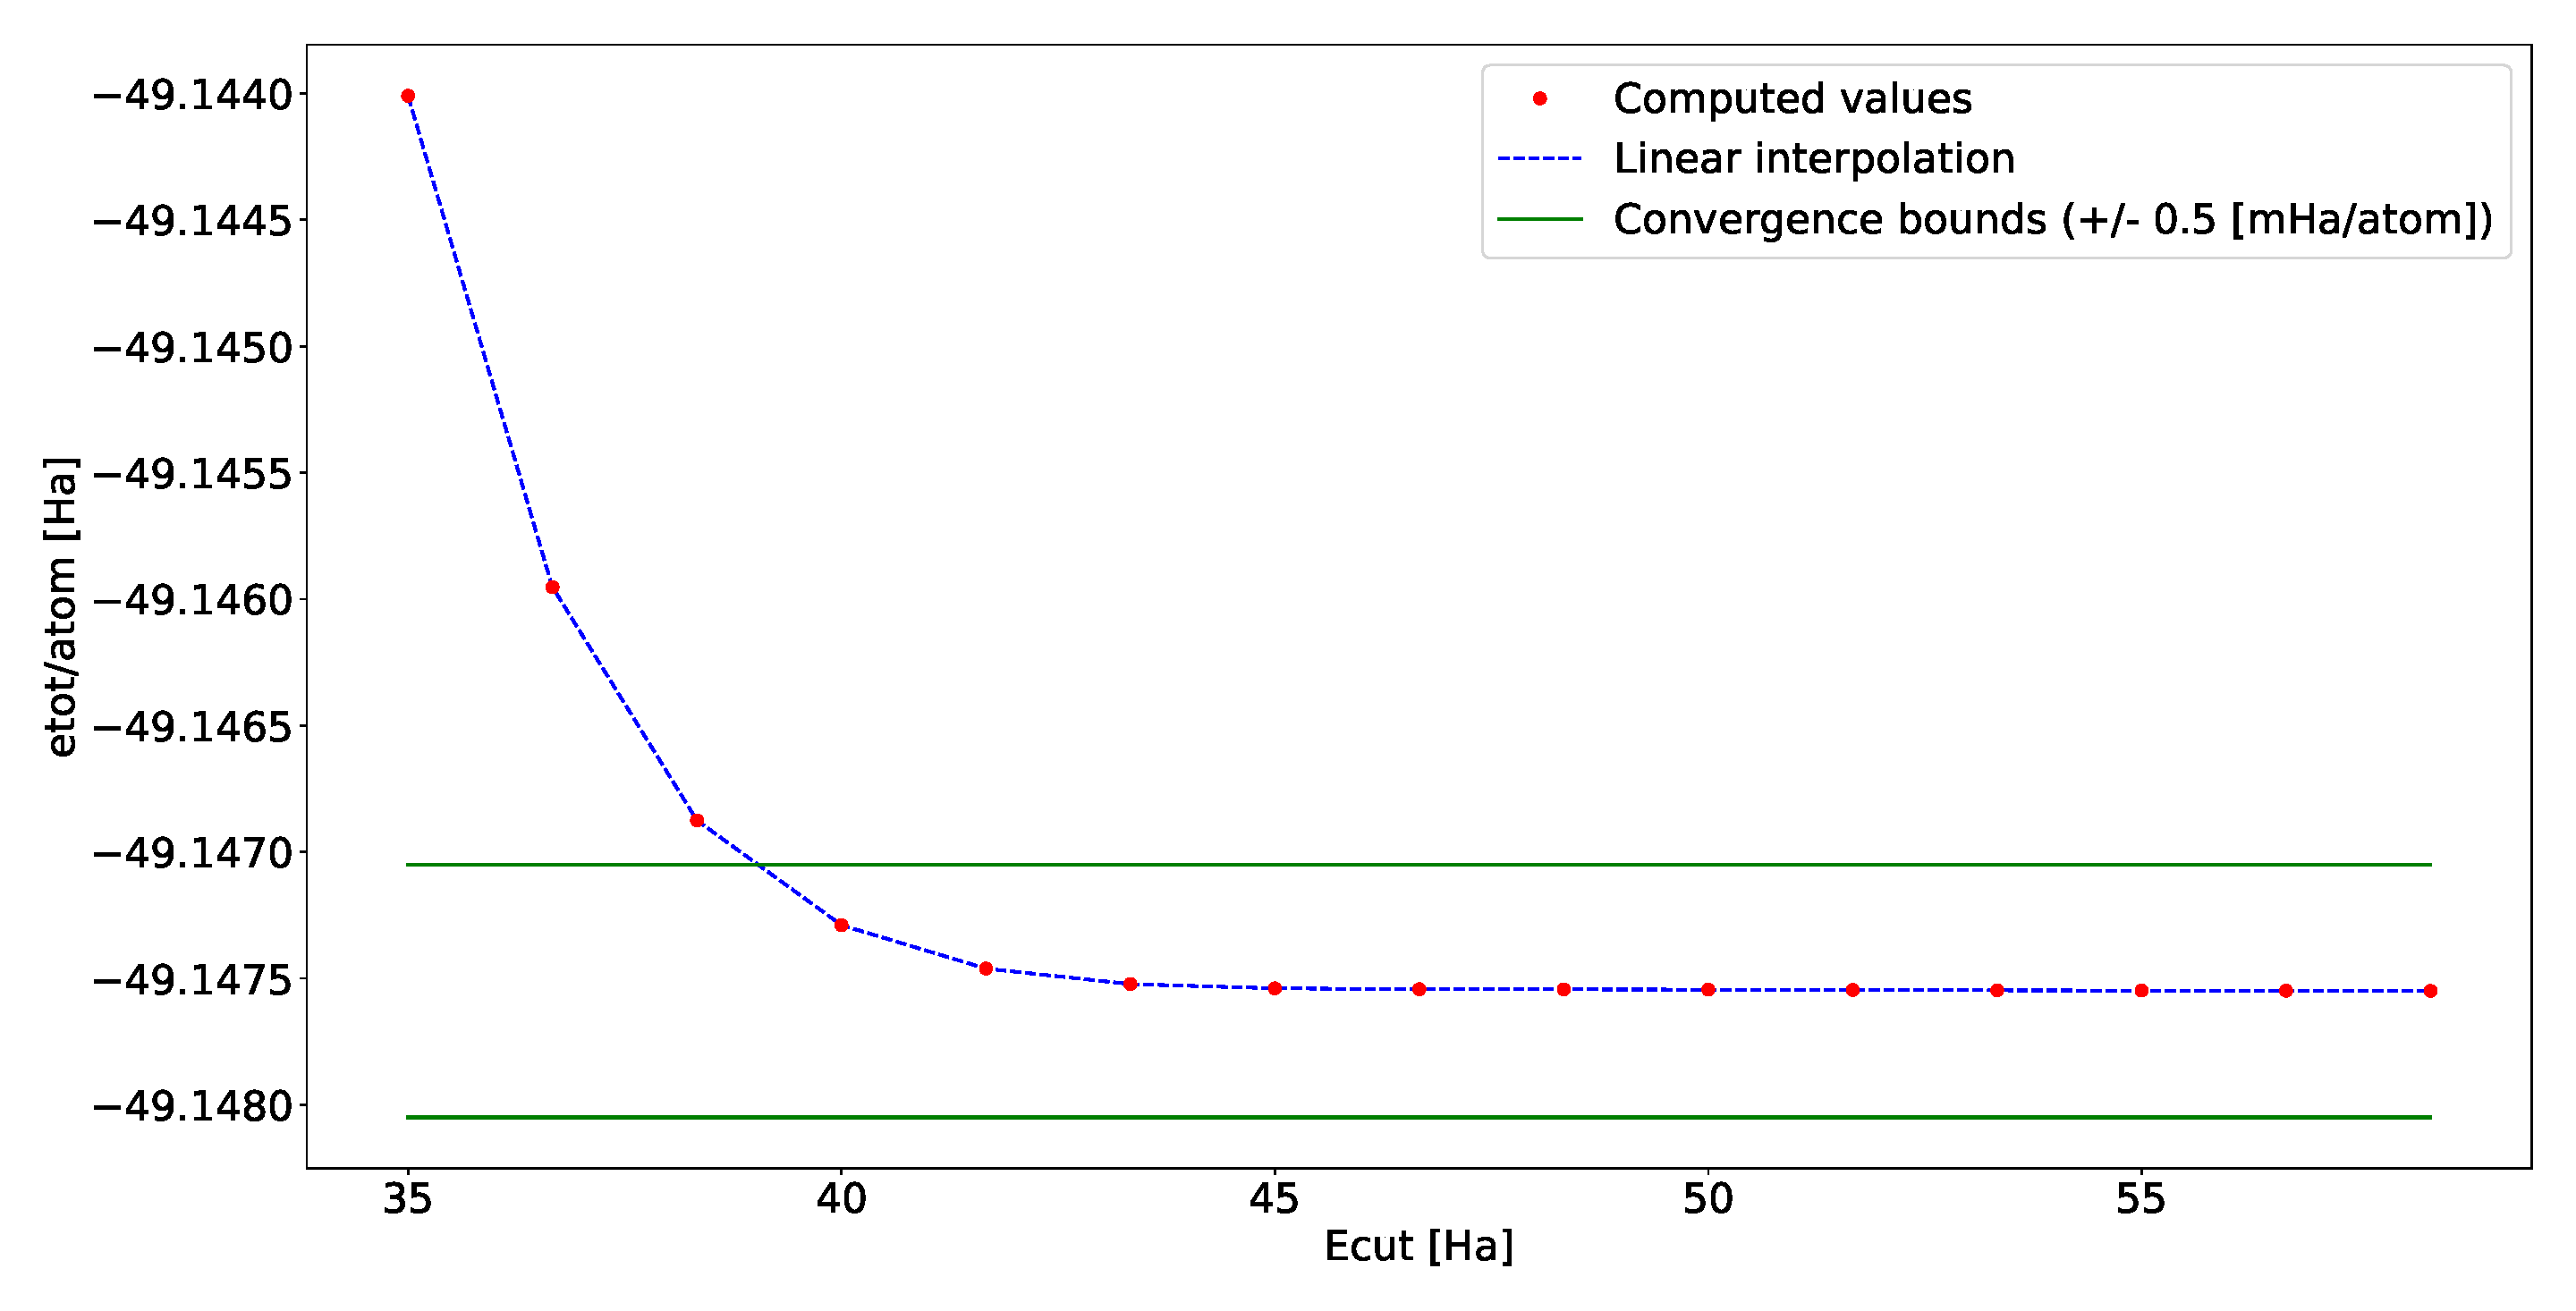
\includegraphics[width=\textwidth]{images/etotecut}
\caption{Total energy per atom as a function of the cut-off energy.\\
The \texttt{ecut} range is truncated for visual reasons.\\
Linear interpolations are shown as a guide for the eyes.}
\label{fig:ecutConv}
\end{figure}

\subsection{Convergence of the total energy per atom as a function of the number of $k$-points (\texttt{ngkpt})}
\label{convEtotNkpt}
Alternatively, the same kind of study is performed with respect to the number of $k$-points in the Brillouin zone. \texttt{Abinit} is run with the input file \texttt{1522\_4\_nkpConv.abi} (\autoref{Abi2}). The energy per atom can be plotted versus the \texttt{ngkpt} parameter (\autoref{fig:nkpConv}).
\begin{figure}[h]
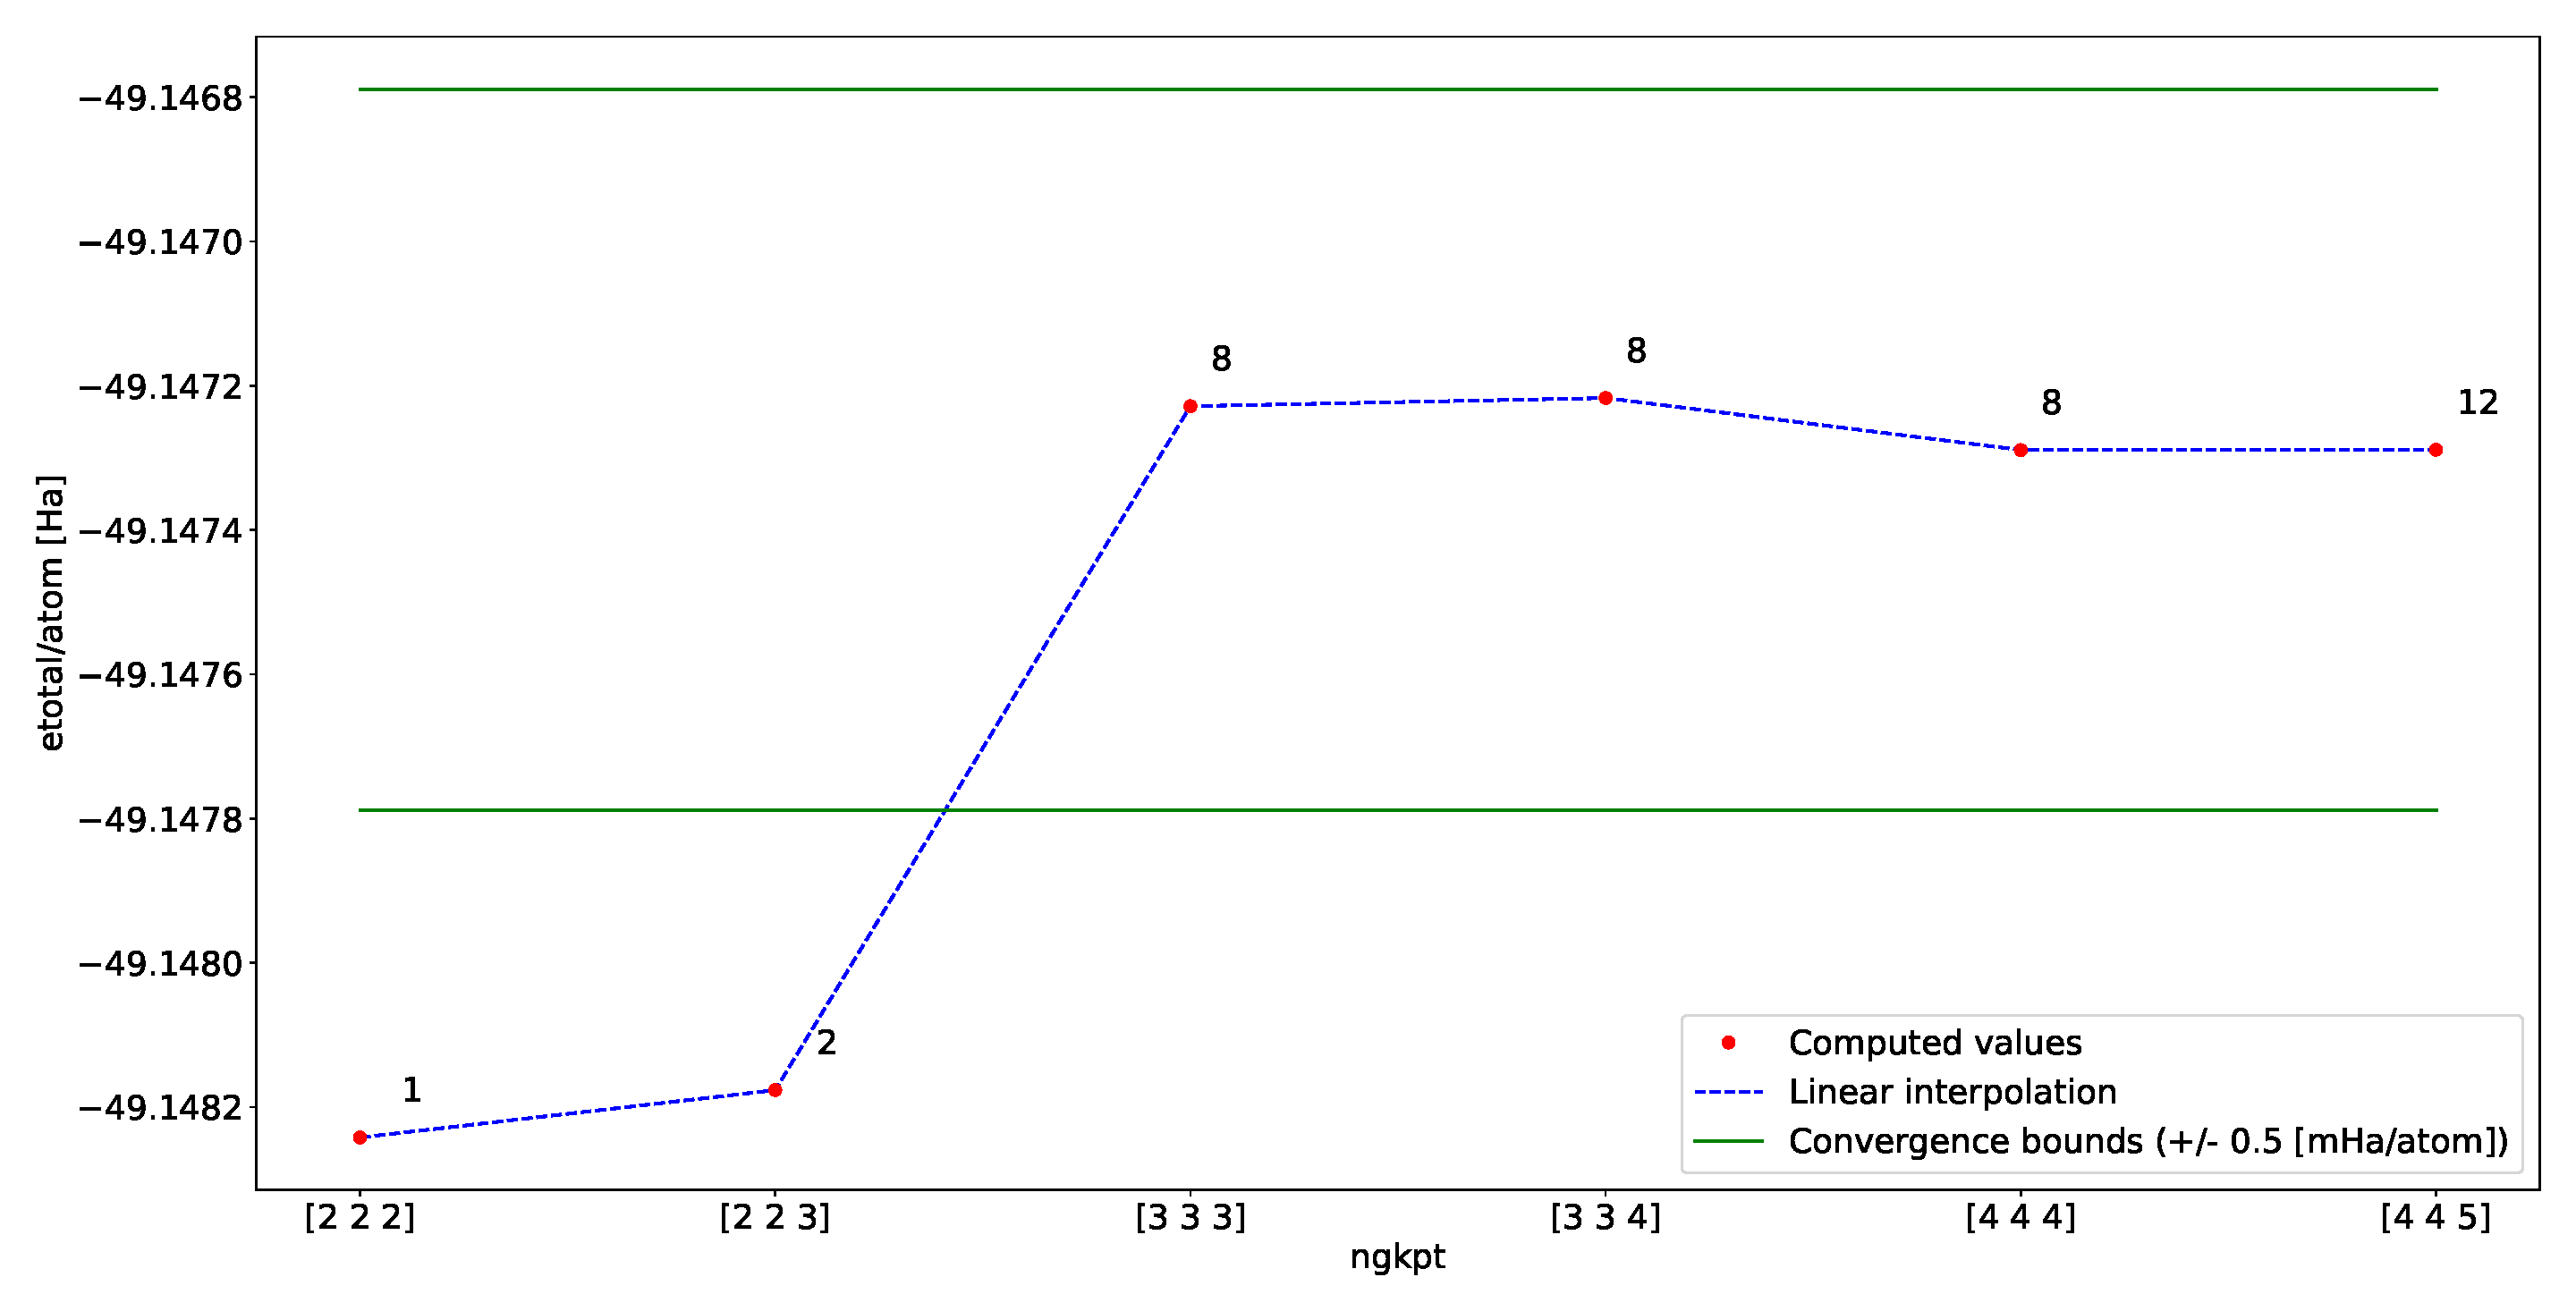
\includegraphics[width=\textwidth]{images/etotngkpt.pdf}
\caption{Total energy per atom as a function of the number of $k$-points in the $k$-points grid.\\
The number near each dot represents the corresponding number of $k$-points.
}
\label{fig:nkpConv}
\end{figure}
However, as the biggest and the smallest lattice scale parameters differs from 60\% in size, additional values of \texttt{ngkpt} keeping a similar $k$-sampling density along each axis are also tested.

The first converged \texttt{ngkpt} value is \texttt{[3 3 3]}.

Concerning the convergence of the total energy per atom, the couple of values (\texttt{ecut},\texttt{ngkpt}) that will be used in the further computations is thus (\texttt{40} [Ha],\texttt{[3 3 3]}).
\subsection{Convergence of \texttt{acell} as a function of the cut-off energy}
The convergence of the length scales of the unit cell was performed using a dataset of \texttt{ecut} values between $20$ [Ha] and $50$ [Ha], \texttt{ngkpt} = \texttt{[3 3 3]} and \texttt{ecutsm} = $0.5$ [Ha]. The input file used is \texttt{1522\_6\_acellEcutConv.abi} (\autoref{Abi3}). The results are displayed on \autoref{fig:acellecutconv}.
The first converged value is $30$ [Ha].
\begin{figure}
\centering
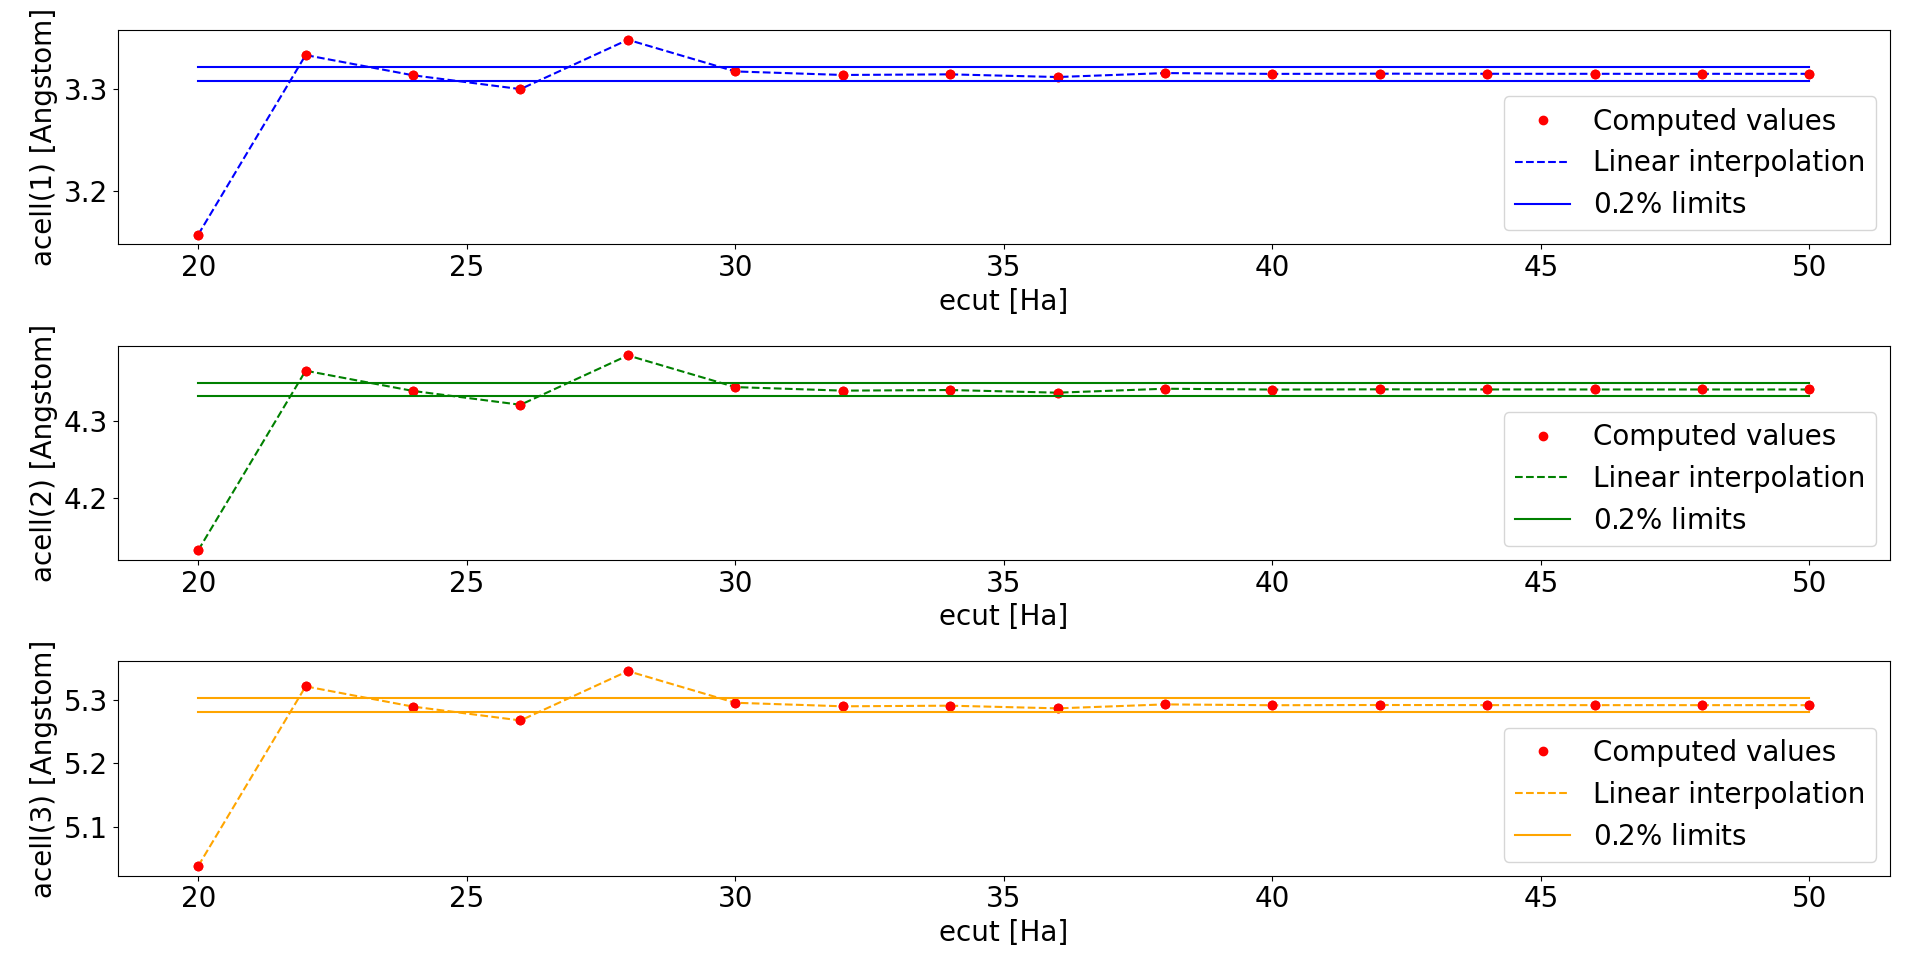
\includegraphics[width=\textwidth]{images/acellConv.png}
\caption{Convergence of the length scales \texttt{acell} as a function of the cut-off energy \texttt{ecut}.}
\label{fig:acellecutconv}
\end{figure}
\subsection{Convergence of \texttt{acell} as a function of the number of $k$-points}
The convergence of the length scales of the unit cell was analyzed with \texttt{ecut} = $40$ [Ha] and \texttt{ecutsm} = $0.5$ [Ha]. Additional values of \texttt{ngkpt} accounting for the conservation of a similar $k$-sampling density along the axis of the unit cell are also tested. The input file used is \texttt{1522\_3\_acellNgkptConv.abi} (\autoref{Abi4}). The results are displayed on \autoref{fig:acellnkpConv}. It can be seen that \texttt{[2 2 2]} is already in the limits of $0.2\%$ of the length. Therefore, the value \texttt{[2 2 2]} is considered as the first converged value.
\begin{figure}
\centering
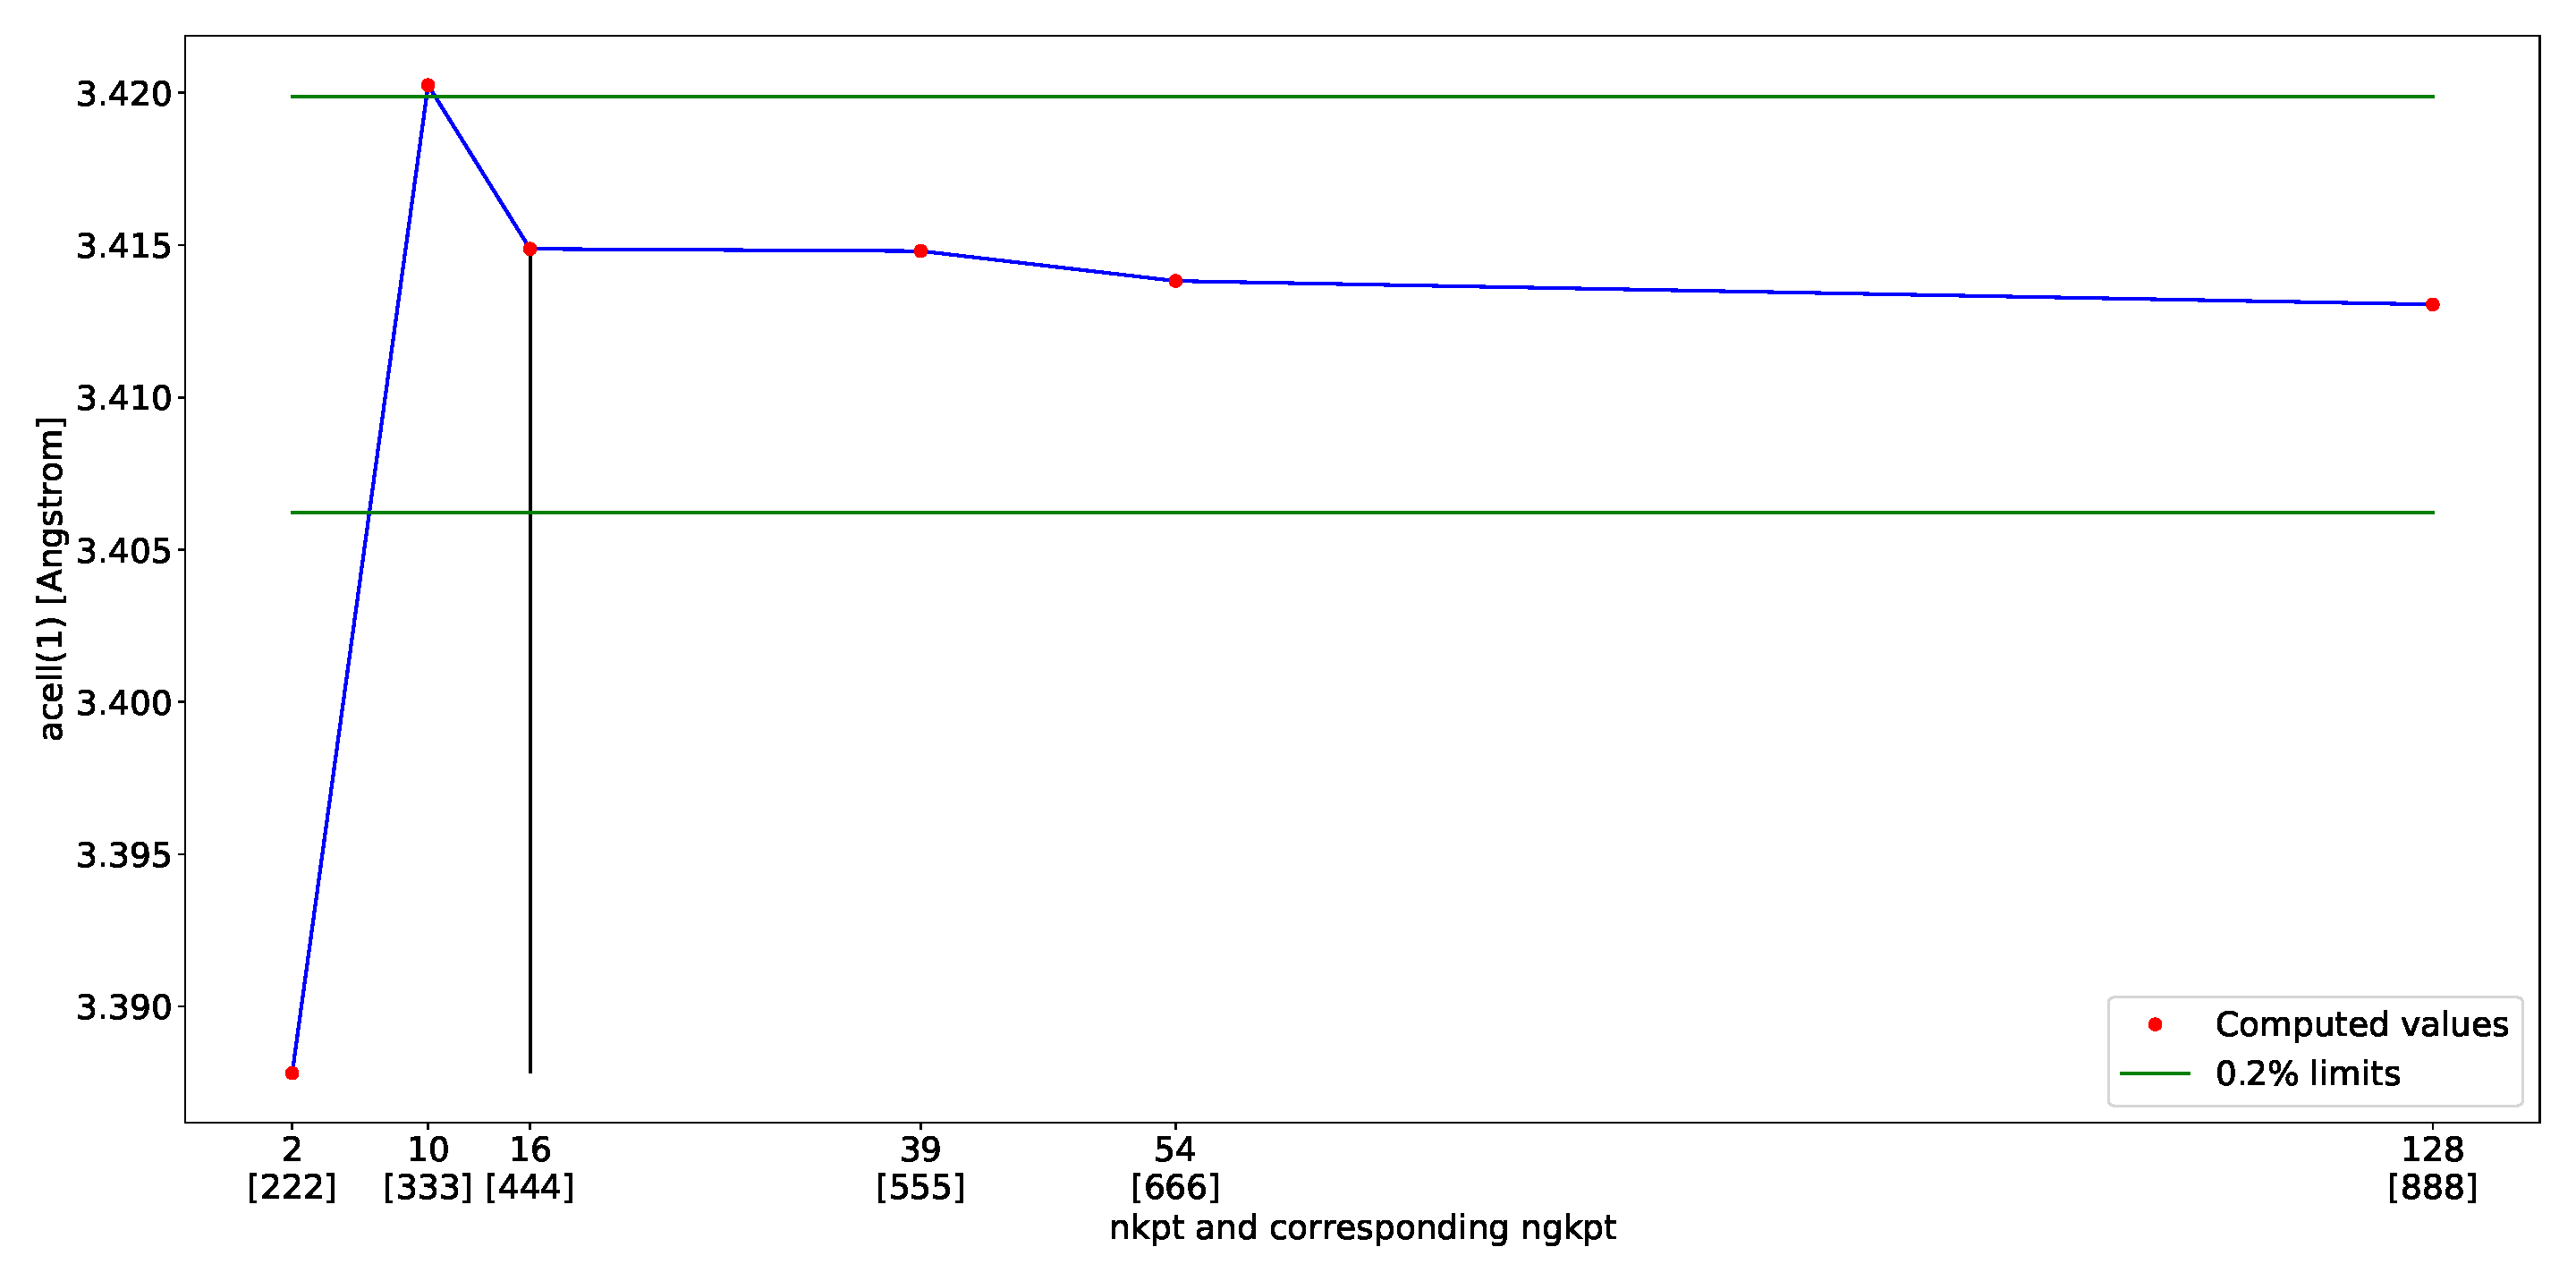
\includegraphics[width=\textwidth]{images/acellNgkpt.pdf}
\caption{Convergence of the length scales \texttt{acell} as a function of the number of $k$-points in the $k$-points grid.
The number near each dot represents the corresponding number of $k$-points.}
\label{fig:acellnkpConv}
\end{figure}
\subsection{Summary}
\begin{center}
\begin{tabular}{|l|c|c|}
\cline{2-3}   
\multicolumn{1}{c|}{}&\texttt{ecut [Ha]} & \texttt{ngkpt} \\
\hline
\multirow{1}{*}{Convergence of \texttt{etotal/atom}} & 40 & [3 3 3]\\
\hline
\multirow{1}{*}{Convergence of \texttt{acell}} & 30 & [2 2 2]\\   
\hline           
\end{tabular}
\end{center}
Furthermore, the most accurate value for \texttt{acell} and \texttt{xred}, obtained with \texttt{ngkpt} = \texttt{[4 4 5]} (\texttt{nkpt} = 12) and \texttt{ecut} = $40$ [Ha], is 
\begin{center}
\begin{tabular}{|c|c|}
\hline 
\texttt{acell(1)} & 6.2645 Bohr\\
\hline
\texttt{acell(2)} & 8.2011 Bohr\\
\hline
\texttt{acell(3)} & 9.9992 Bohr\\
\hline
\end{tabular}
\end{center}
or
\begin{center}
\begin{tabular}{|c|c|}
\hline
\texttt{acell(1)} & 3.315 Angstroms\\
\hline
\texttt{acell(2)} & 4.3398 Angstroms\\
\hline
\texttt{acell(3)} & 5.2913 Angstroms\\
\hline
\end{tabular}
\end{center}
and
\begin{center}
\begin{tabular}{|l|c|c|c|}
\cline{2-4}
\multicolumn{1}{l|}{}&\texttt{xred(1)} & \texttt{xred(2)} & \texttt{xred(3)}\\
\hline
\texttt{Fe \#1} & 0 & 0 & 0 \\
\hline
\texttt{Fe \#2} & 0.5 & 0.5 & 0.5\\
\hline
\texttt{S \#1} & 0 & 2.0809E-01 & 3.7374E-01\\
\hline
\texttt{S \#2} & 0& 7.9191E-01 & 6.2626E-01\\
\hline
\texttt{S \#3} & 0.5 & 2.9191E-01 & 8.7374E-01\\
\hline
\texttt{S \#4} & 0.5 & 7.0809E-01 & 1.2626E-01\\
\hline
\end{tabular}
\end{center}
\section{Optical properties}
\subsection{Electronic band structure}
\label{elecbs}
The band structure of the material was computed as follows. First, an optimal $k$-path is generated in the Brillouin zone of a simple orthorhombic lattice \autoref{fig:orcBZ} using the \texttt{Abistruct} module of \texttt{Abipy} (\autoref{Abi5}). 

\begin{figure}[h]
\centering
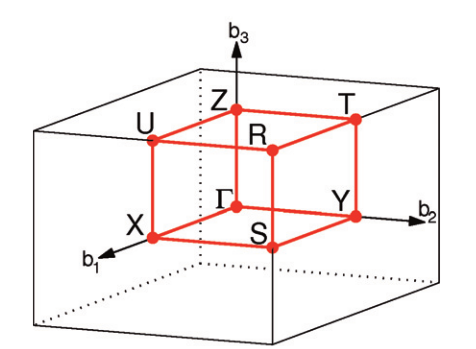
\includegraphics[width=0.4\textwidth]{images/bz.png}
\caption{Brillouin zone for a simple orthorhombic lattice \cite{bz}}
\label{fig:orcBZ}
\end{figure}

To obtain the band structure of the material, a SCF computation of the electronic density is run in the first place. Then, the band structure is computed using a non-SCF computation based on the previously generated electronic density file. The structural parameters of the unit cell are the ones provided by \texttt{Absitruct}. \texttt{ecut} and \texttt{ngkpt} are chosen accordingly to the previous convergence studies.

For the SCF computation, \texttt{prtden} is set to \texttt{1}, in order to generate the DEN files.

For the band structure computation, \texttt{iscf} is set to \texttt{-2} and \texttt{getden} is set to \texttt{-1} to read the electronic densities from the previously generated DEN file.
As the pseudopotentials used only consider 56 electrons in the whole unit cell, 27 electronic bands are completely filled. The 28th band is thus the valence band. To obtain a clear representation of the band gap of the material, 35 electronic bands are defined. \texttt{kptopt} is set to \texttt{-15} accrodingly to the $k$-path provided by Abistruct. \texttt{ndivsm} is set to \texttt{30}, and \texttt{nbdbuf} is set to \texttt{-2} to place the last 2\% bands of highest energy in a buffer, preventing \texttt{Abinit} to spent too much time trying to converge them.

The input file \texttt{1522\_14\_bs.abi} is available in \autoref{Abi6}. 



The band structure is represented on \autoref{fig:bs}. The Fermi energy and the energy of the bandgap were also retrieved from the computed data. It is compared below with the data from the Materials Project \cite{MaterialsProject}. The band structure provided by the Materials Project, which can be found in \autoref{Abi7}, is compared with the computed one on \autoref{fig:bsMPCombined}.

Besides a difference of $2.45$ eV concerning the Fermi energies, the results of the computation seems consistent regarding the data of the Materials Project. That difference can be explained by a difference in the value of the parameters ruling the computation. 
\begin{table}
\centering
\begin{tabular}{|l|c|c|}
\cline{2-3}
\multicolumn{1}{l|}{}&\textbf{Computed}&\textbf{Materials Project}\\
\hline 
\textbf{Fermi energy [eV]}& $10.13183$&$7.6763$\\
\hline
\textbf{Band gap energy [eV]} & $0.8674$ & $0.8807$ \\
\hline
\end{tabular}
\caption{Comparison between the computed results and the data provided by the Materials Project}
\label{tab:bg}
\end{table}
\begin{figure}[h]
\centering
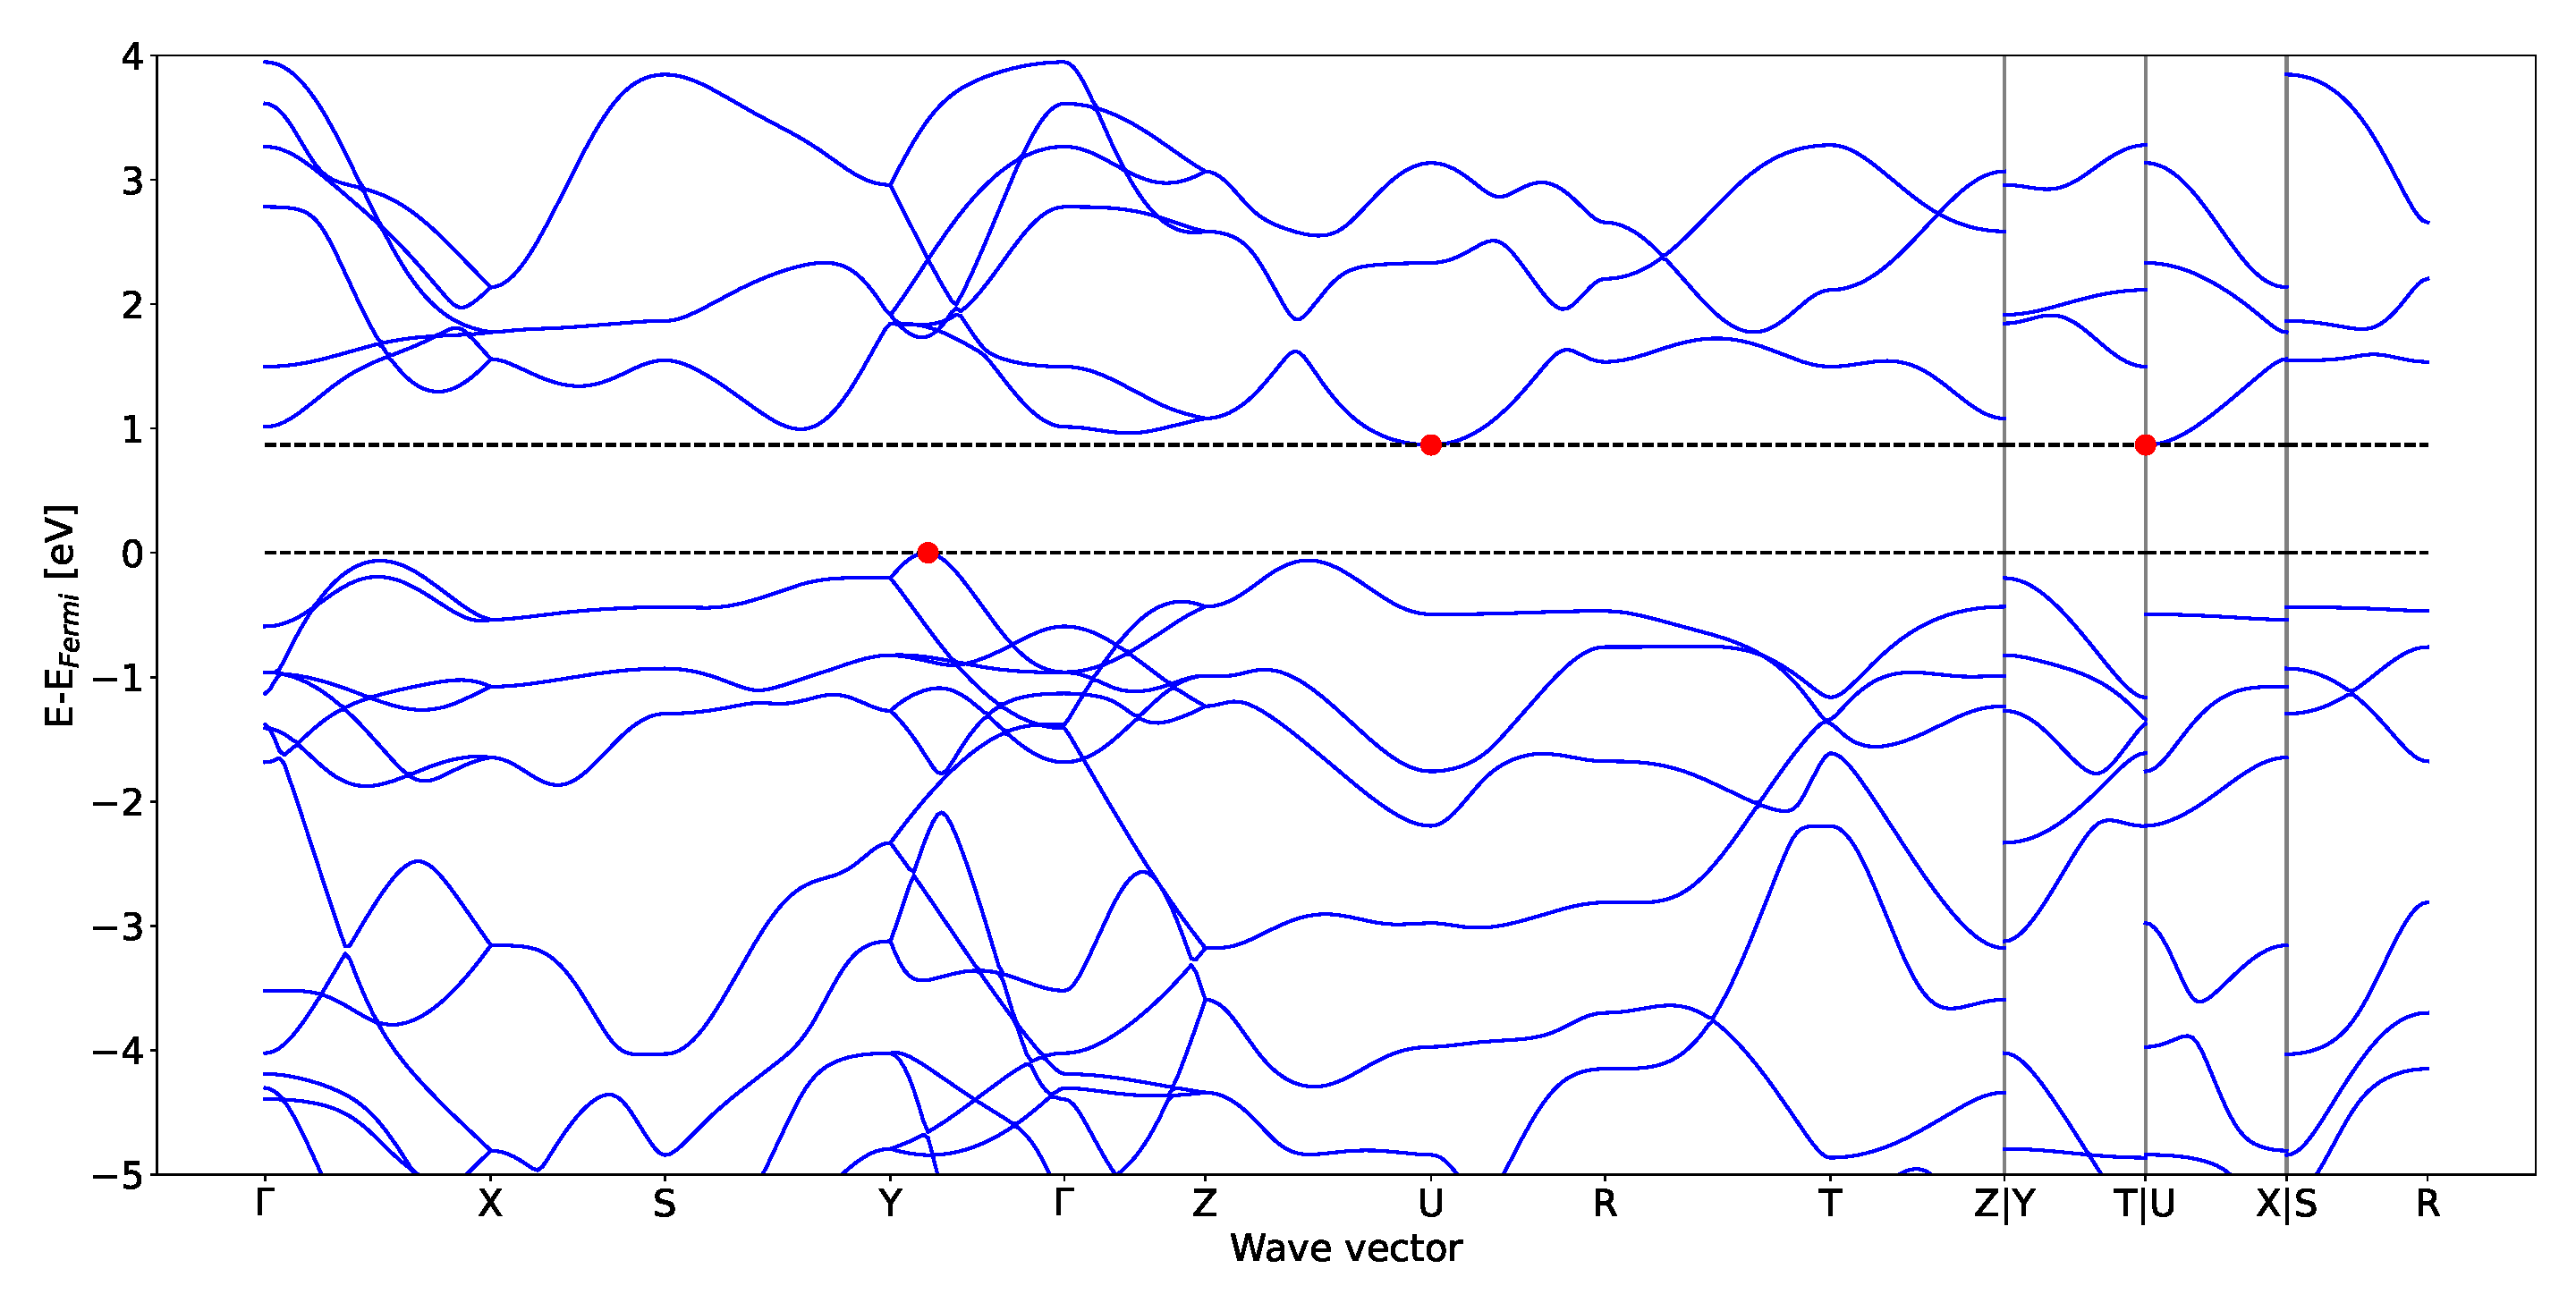
\includegraphics[width=\textwidth]{images/bs.pdf}
\caption{Band structure of \ch{FeS2}. The red dots represent the valence band minimums and the conduction band maximum.}
\label{fig:bs}
\end{figure}
\begin{figure}
\centering
\includegraphics[width=\textwidth]{images/bsCombined.pdf}
\caption{Blue : Band structure provided by the Materials Project. Red : Computed band structure.}
\label{fig:bsMPCombined}
\end{figure}
\subsection{Electronic density of states (DOS)}
The electronic density of states was obtained by first running a SCF computation to generate a density file as for the computation of the bandstructure. In that case, \texttt{shiftk} was set to \texttt{[0 0 0]} as recommended in the Abinit documentation \cite{AbinitManual}.

Then, the DOS was computed using the tetrahedron methode with \texttt{prtdos} = \texttt{2} and \texttt{dosdeltae} = \texttt{5.0d-5} Ha. \texttt{ngkpt} was set to \texttt{[8 8 8]} to ensure a good resolution in the DOS plot. The input file used is available in \autoref{Abi8}. Several plots were obtained when trying to display the density of states of the material. Each of the plot presents a different level of smearing. The smearing is controlled by the $k$-sampling of the Brillouin zone and the step of energy that was chosen during the computation of the density of states. Indeed, the $k$-sampling and the energy step have both an influence on the resolution of the plot, as the DOS plot is obtained with the sum of Gaussian spreads localized on the eingenvalues composing each band, and for each $k$-point. Therefore, the smaller the energy step, the more detailed (and as it will be seen, the rougher) the pattern of density of states, as long as the $k$-sampling is sufficiently high (if the number of $k$-points or the energy step is too small, there will be undesired gaps in the DOS plot).
 
By default, \texttt{Abipy} smears the the plot of the DOS, no matter what step of energy was chosen fort the computation. It will thus be compared to the DOS pattern provided by the Materials Project, as the smearing is of the same order of magnitude there. The comparison is displayed on \autoref{fig:dosSmeared}. It can be seen that the two plots present the same features : a drop of the DOS at $E = 0$ eV representing the bandgap, and similar peaks around the bandgap. However, substantial differences subsist : 
\begin{itemize}
\item First, the plot displayed by \texttt{Abipy} (\autoref{fig:dos1}) isn't as wide as the one provided by the Materials Project (\autoref{fig:dos4}). This is due to the fact that only the first conduction band was computed with \texttt{Abinit} in the first case, while additional conduction bands were considered on the Materials Project.
\item Secondly, the amplitude of the peaks isn't the same for the two graphs. Once again, it is presumably due to smearing reasons. The main drawback of these two sources (\texttt{Abipy} and the Materials Project) is that the smearing (or the energy step and the sampling of the Brillouin zone) is a black box. However, it can also be due to the method that was used to generate the data (but as it is not specified on the Materials Project, it's difficult to be sure).
\item Lastly, it can be seen that the peaks on the plot provided by the Mateirals Project are higher in terms of DOS than on the plot calculated by \texttt{Abinit} and displayed by \texttt{Abipy}. That difference can be explained by a difference between the smearing level and the $k$-points lattice that has been chosen to run the computation. However, the most worthwhile comparison concerns the density of valence states.
\end{itemize}
\begin{figure}[H]
\centering
\begin{subfigure}[b]{0.95\textwidth}
\centering
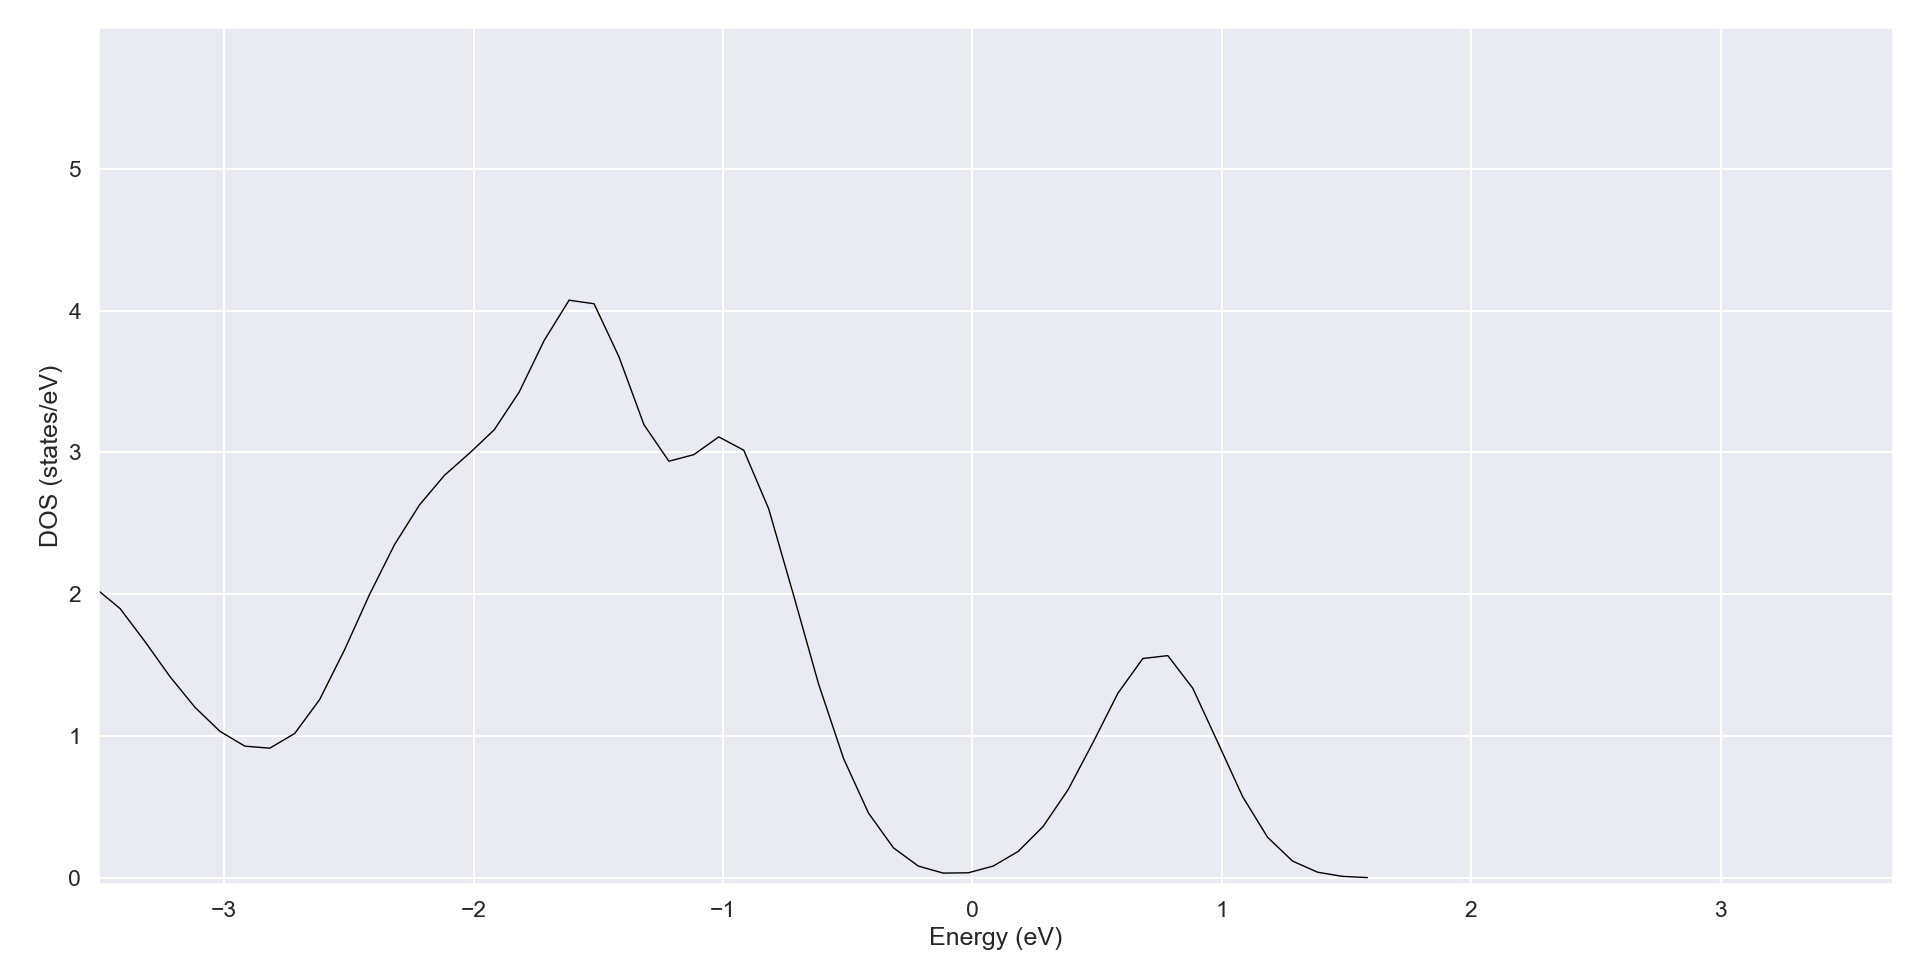
\includegraphics[width=\textwidth]{images/dos1}
\caption{Electronic DOS (displayed using \texttt{Abipy})}
\label{fig:dos1}
\end{subfigure}

\begin{subfigure}[b]{0.95\textwidth}
\centering
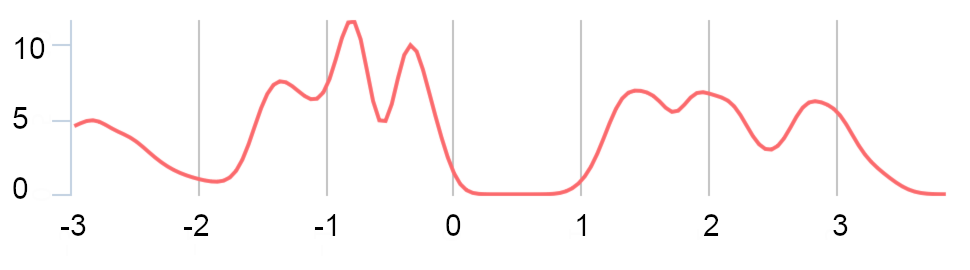
\includegraphics[width=\textwidth]{images/dos4.png}
\caption{Electronic DOS provided by the Materials Project (\url{https://materialsproject.org/materials/mp-1522/})}
\label{fig:dos4}
\end{subfigure}
\caption{Comparison of the most smeared DOS patterns}
\label{fig:dosSmeared}
\end{figure}

Then, the plot of the electronic DOS was displayed using a handmade \texttt{Python} script, using the \texttt{\_DS2\_GSR.nc} output file generated by \texttt{Abinit} (here \texttt{DS2} is explained by the fact that the DOS was computed in the second dataset of the run, the first one being the SCF density computation). It was then compared with a plot of the DOS whose smearing seems to be significantly lower than for the two previous examples. The latter plot was obtained on the Topological Materials Database \cite{TMD1,TMD2,TMD3,TMD4,TMD5}.  The two plots are compared on \autoref{fig:dosLessSmeared}. The goal here is to make the comparison between two less smeared plots.

\begin{figure}[H]
\centering
\begin{subfigure}[b]{0.57\textwidth}
\centering
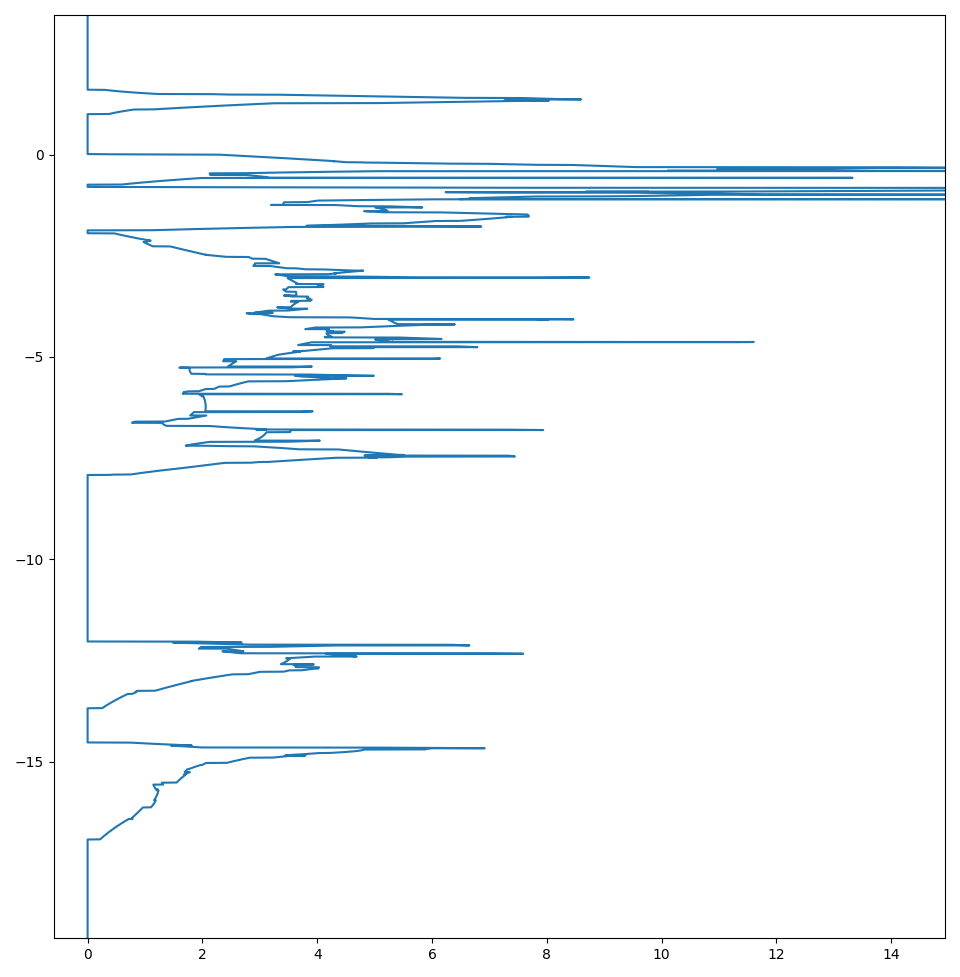
\includegraphics[width=\textwidth]{images/dos2}
\caption{Electronic DOS plotted using \texttt{Python} and the \texttt{\_DS2\_GSR.nc Abinit} output file\\\hspace{1cm}\\}
\label{fig:dos2}
\end{subfigure}
\hfill
\begin{subfigure}[b]{0.33\textwidth}
\centering
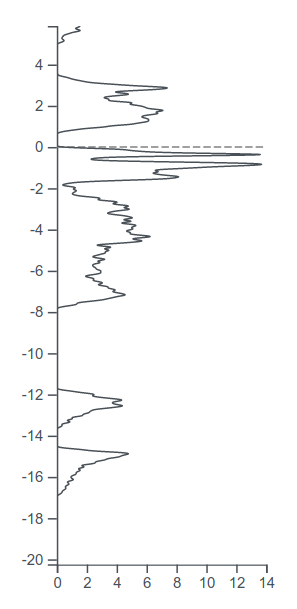
\includegraphics[width=\textwidth]{images/dos3.png}
\caption{Electronic DOS provided by the Topological Materials Database}
\label{fig:dos3}
\end{subfigure}
\caption{Comparison of less smeared DOS patterns}
\label{fig:dosLessSmeared}
\end{figure}

One can see here that the plots also show the same features. Some differences can however be mentioned : 
\begin{itemize}
\item On the plot obtained using \texttt{Abinit} and \texttt{Python} (\autoref{fig:dos2}), the peaks above the bandgap are not as developed as on the plot provided by the Topological Materials Database (\autoref{fig:dos3}). This is due to the same reason as previously : only the first conduction band has been considered during the \texttt{Abinit} computation, while it is clearly not the case for the other plot. 
\item On the plot obtained with \texttt{Python}, peaks of high amplitude can be seen at several energies (for example just below the bandgap). After further investigation, the peaks span until a DOS of $\sim$ 65 states/eV, implying that the amplitude of those peaks is probably a computational artefact. Such peaks are not visible on the other plot, because it has been smeared a little, demonstrating the utility of the smearing of the plot of the electronic DOS.
\end{itemize}
\subsection{Phonon dispersion}
The phonon dispersion of the material was computed as follows. First, a list of convenient $q$-points has to be generated. This is done by generating a list of $k$-points. To do so, we run a standard SCF computation. However in this case the SCF procedure is dummy. Indeed, \texttt{nstep} and \texttt{nline} are set to \texttt{1}, preventing \texttt{Abinit} to run more than one iteration during the computation, as explained in \cite{tutoPhonons}. The input file is available in \autoref{Abi9}. Note that \texttt{shiftk} was set to \texttt{[0 0 0]} and not \texttt{[0.5 0.5 0.5]} as in the previous computations. This is done to force \texttt{Abinit} to include the $\Gamma$ point in the list to be generated.

Once the list of $k$-points is generated, we use it as a list of $q$-points for the further computations. The next step is to compute the phonon spectrum over the obtained $q$-points. A few datasets are used : 
\begin{itemize}
\item The first one is a ground-state self-consistency computation that will be used for all the other datasets. 
\item The second dataset is used to compute the response function of the ground-state wavefunctions with respect to $k$ ($\frac{\text{d}}{\text{d}k}$ calculation).
\item The third one is used to compute the response function at $\Gamma$ of an electric field perturbation.
\item The other datasets are used to compute the phonon response at the other $q$-points. As only one $q$-point can be considered at a time, we need as many additional datasets as $q$-points.
\end{itemize}
After the run, several databases are generated, corresponding to the specified datasets. The input file is available in \autoref{Abi10}. Those databases are merged and analyzed using the \texttt{MRGDDB} and \texttt{ANADDB} utilities. During the latter analysis, \texttt{ANADDB} computes different physical properties based on the databases containing the derivatives of the total energy (merged using \texttt{MRGDDB}). The properties to be computed are specified by a series of \textit{flags}. For example : 
\begin{itemize}
\item \texttt{ifcflag} is used to compute the interatomic force constants, which will be used to interpolate the phonon spectrum used in the band structure.
\item \texttt{dipdip} is used to handle the dipole-dipole interactions separately from the interatomic forces, leading to more accurate results.
\item \texttt{eivec} is used to generate an output file containing the frequencies for the different $q$-points, allowing to plot the phonon dispersion (refered to as the \texttt{\_B2EPS.freq} file).
\item \texttt{prtdos} allows to output a file containing the phonon density of states (see \autoref{fig:phonondos}).
\end{itemize}
The input file must also contain two specific lists of $q$-points. The first one is the $q$-path along which the phonon dipsersion will be computed. A previous list of $k$-points used to plot the electronic band structure was used. The second list of $q$-points contains actually one single $q$-point : $\Gamma$. Indeed, a discontinuity can be seen in the phonon band structure at this specific point. The frequencies computed at this point will be hardcoded in the \texttt{\_B2EPS.freq} file to get a proper plot\footnote{Note that the discontinuity at $\Gamma$ is still there on \autoref{fig:phonon1} and \autoref{fig:phonon2}. Indeed, no package was able to open the hacked \texttt{.eps} file properly.}.

Then, using the generated \texttt{\_B2EPS.freq} file containing the frequencies for all the $q$-points of the specified $q$-path, it is possible to produce a final file containing the band structure. It was plotted using \texttt{Abipy} (\autoref{fig:phonon1}) and was compared with the phonon dispersion plot provided by the Materials Project (\autoref{fig:phonon2}).
\begin{figure}
\centering
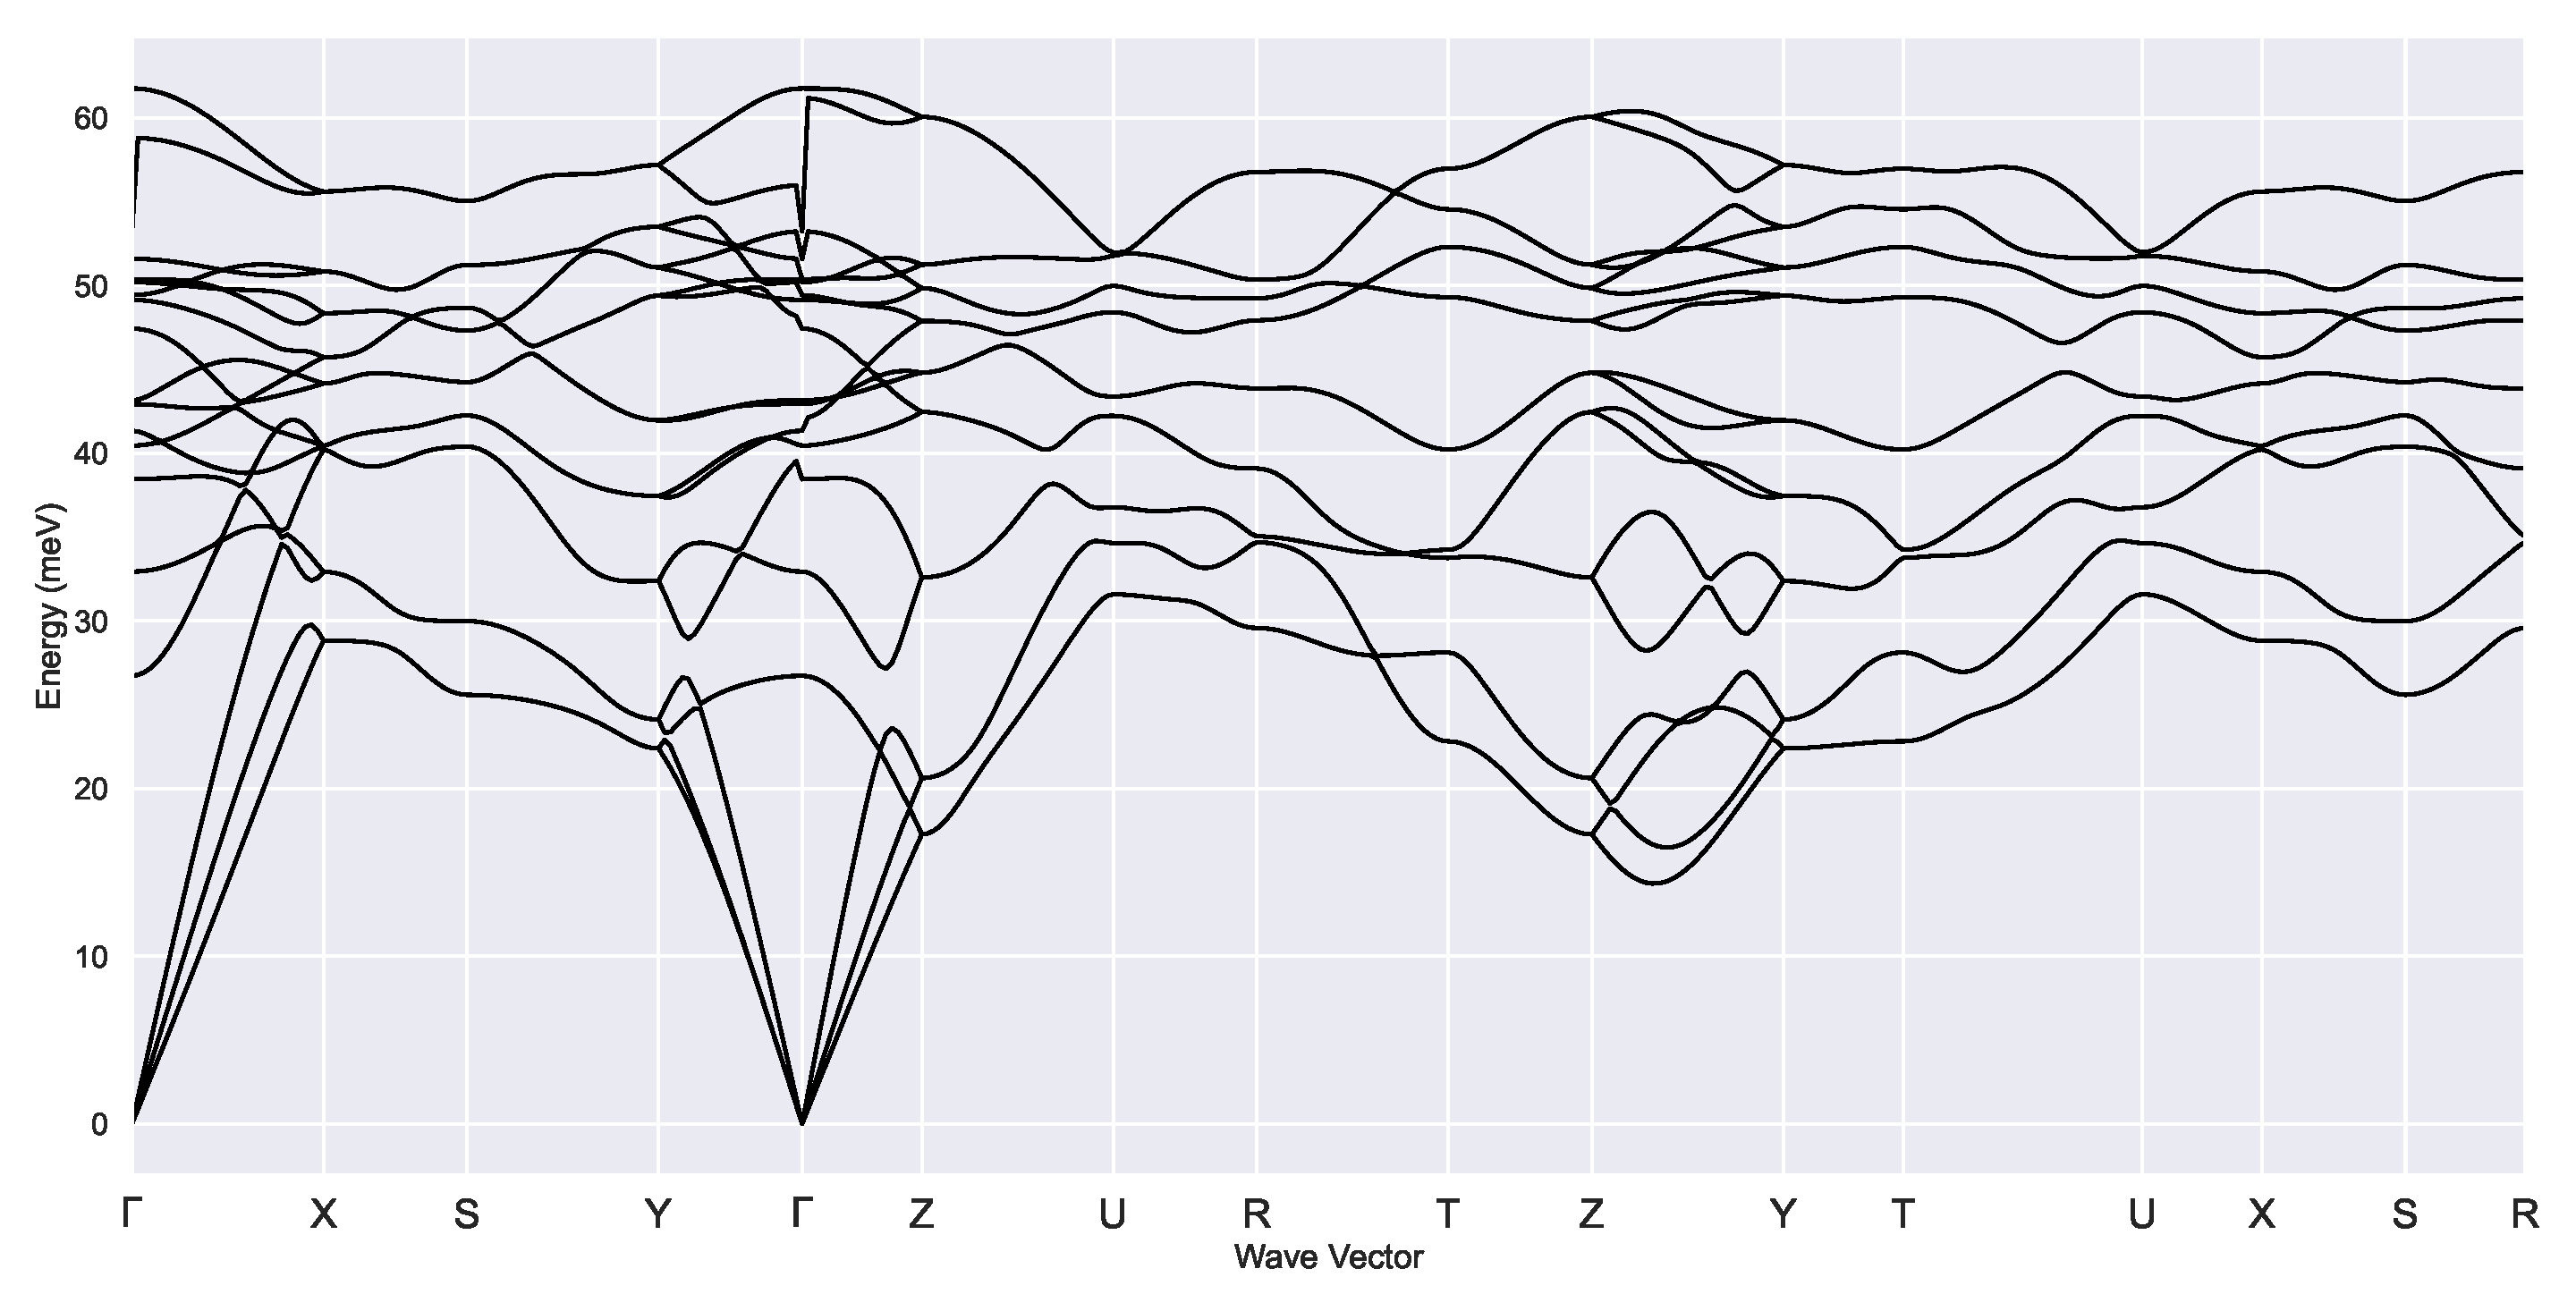
\includegraphics[width=\textwidth]{images/phonon1.pdf}
\caption{Computed phonon dispersion plotted with \texttt{Abipy}}
\label{fig:phonon1}
\end{figure}

\begin{figure}
\centering
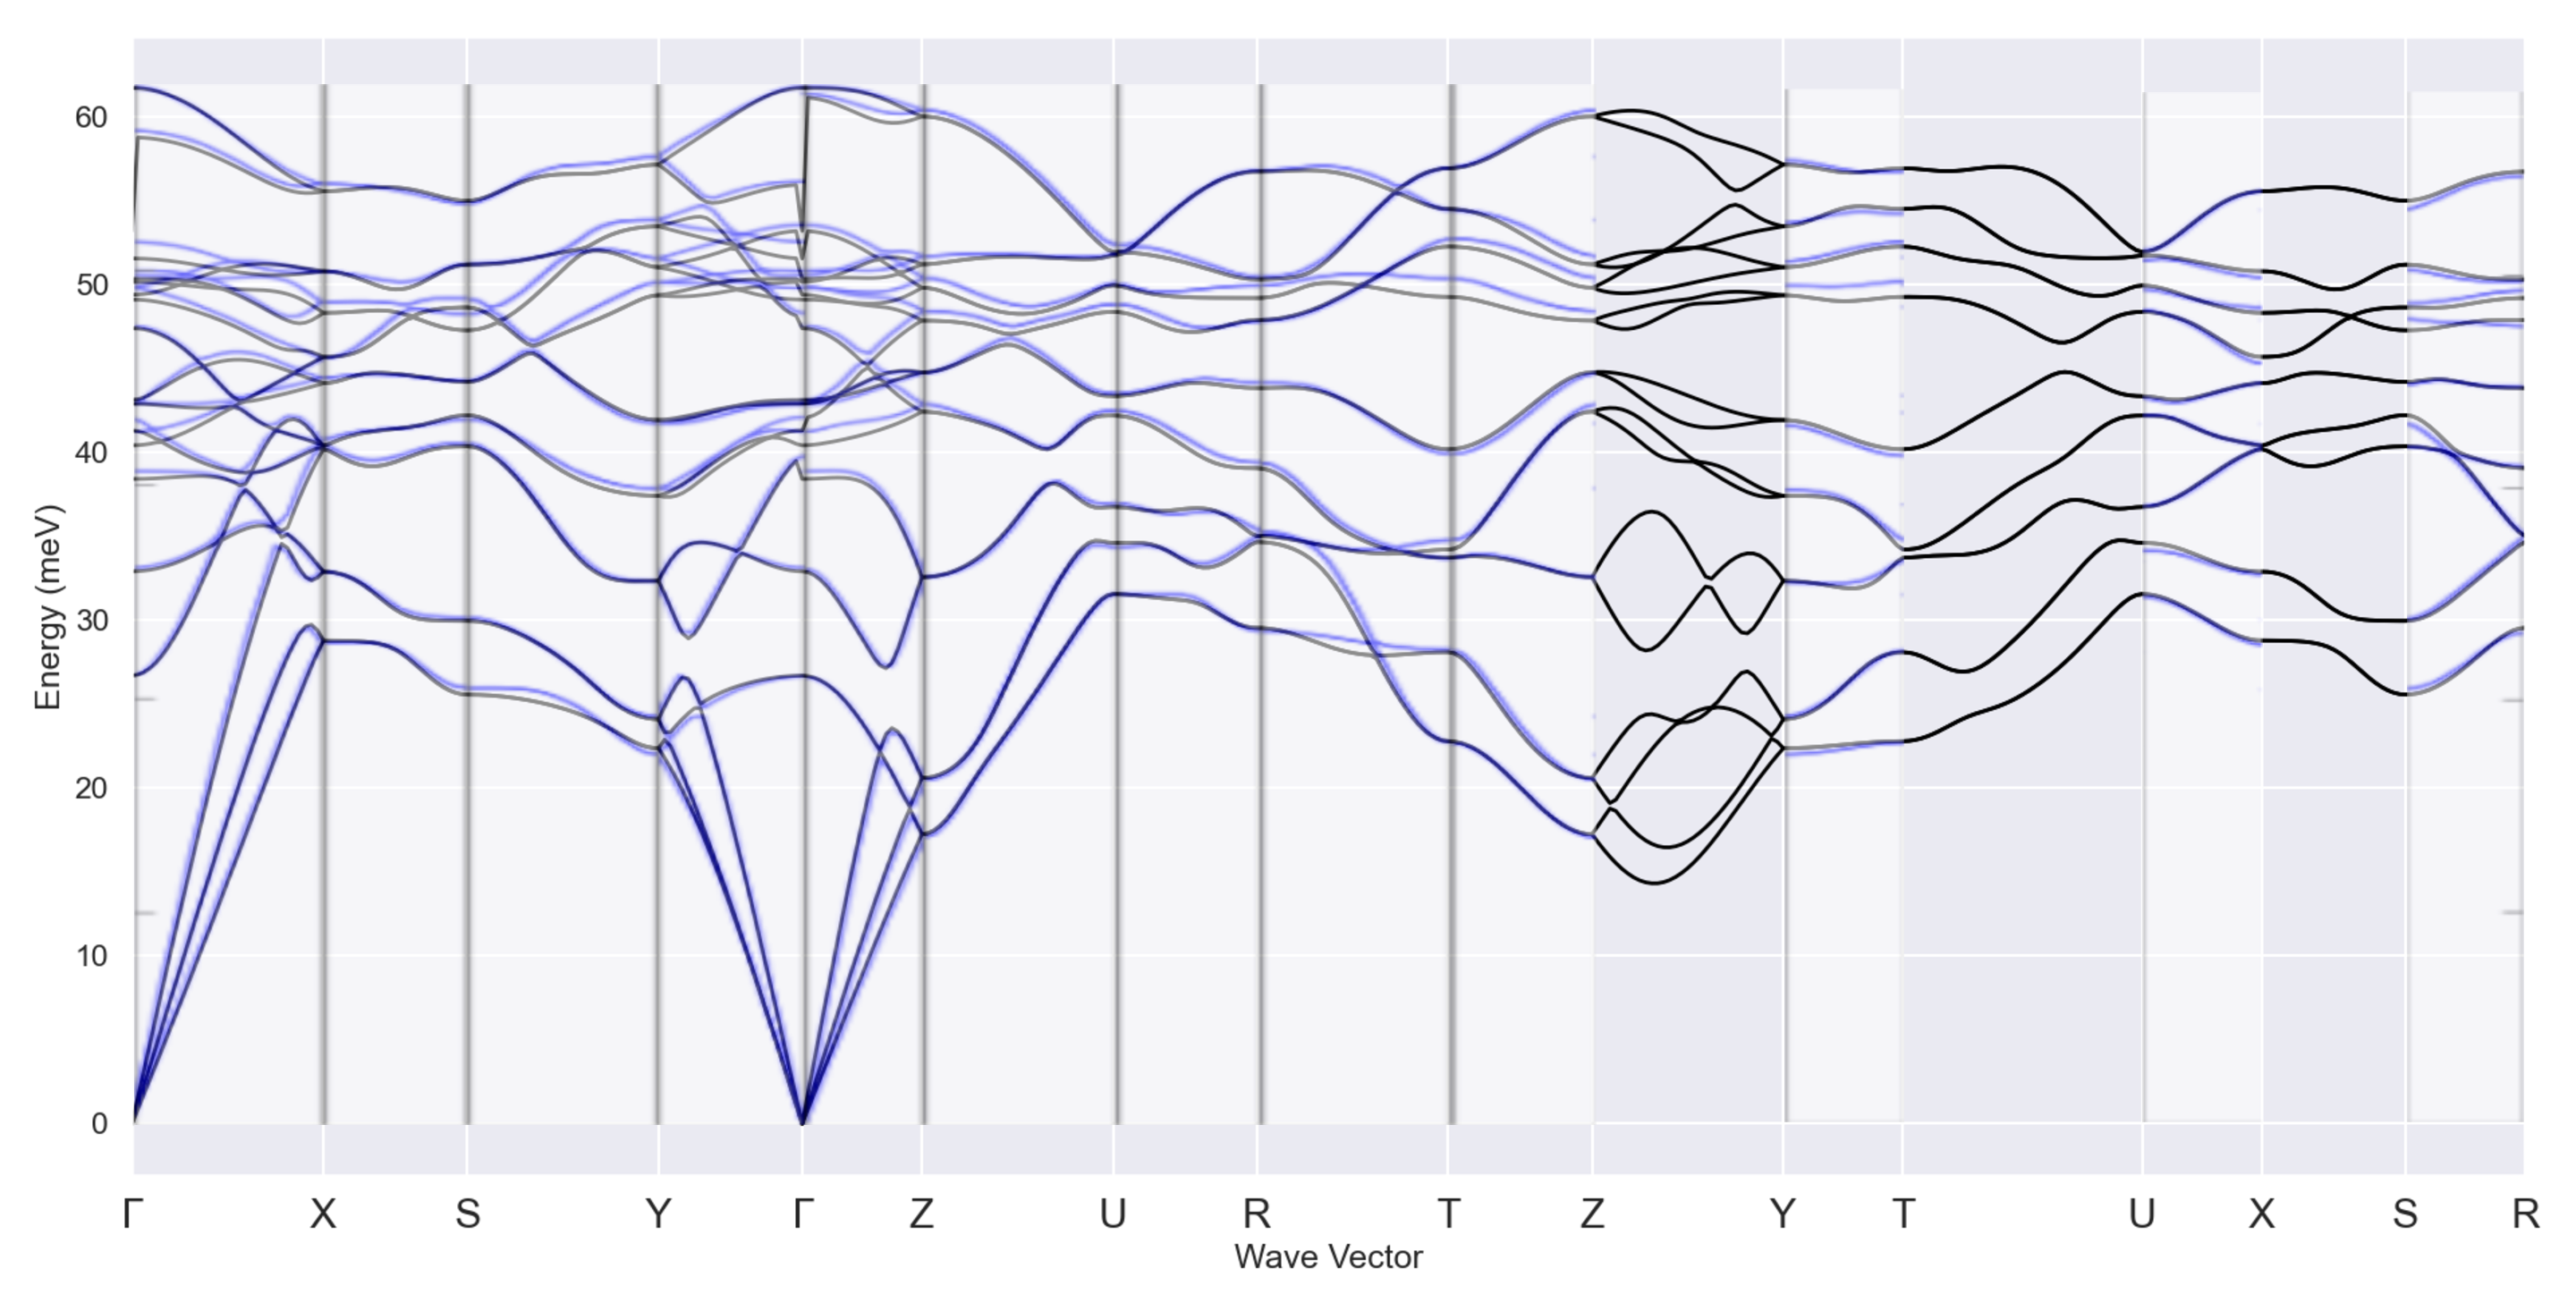
\includegraphics[width=\textwidth]{images/phonon2.pdf}
\caption{Comparison between the computed phonon dispersion (in black) and the phonon dispersion obtained on the Materials Project (in blue, \url{https://materialsproject.org/materials/mp-1522/}). The superposition of the plots is not complete as the plot provided by the Materials Project is truncated at some $q$-points.}
\label{fig:phonon2}
\end{figure}

\subsection{Phonon density of states}
By setting \texttt{prtdos = 2}, it is possible to compute the phonon DOS using the tetrahedron method. The plot is obtained with \texttt{Abipy}, and is compared in \autoref{fig:phonondos} with the phonon DOS plot provided on the Materials Project. It can be seen that the results are in good agreement, as the plots show the same features, and only differ by the smearing level of the plot.

\begin{figure}
\centering
\begin{subfigure}[b]{0.55\textwidth}
\centering
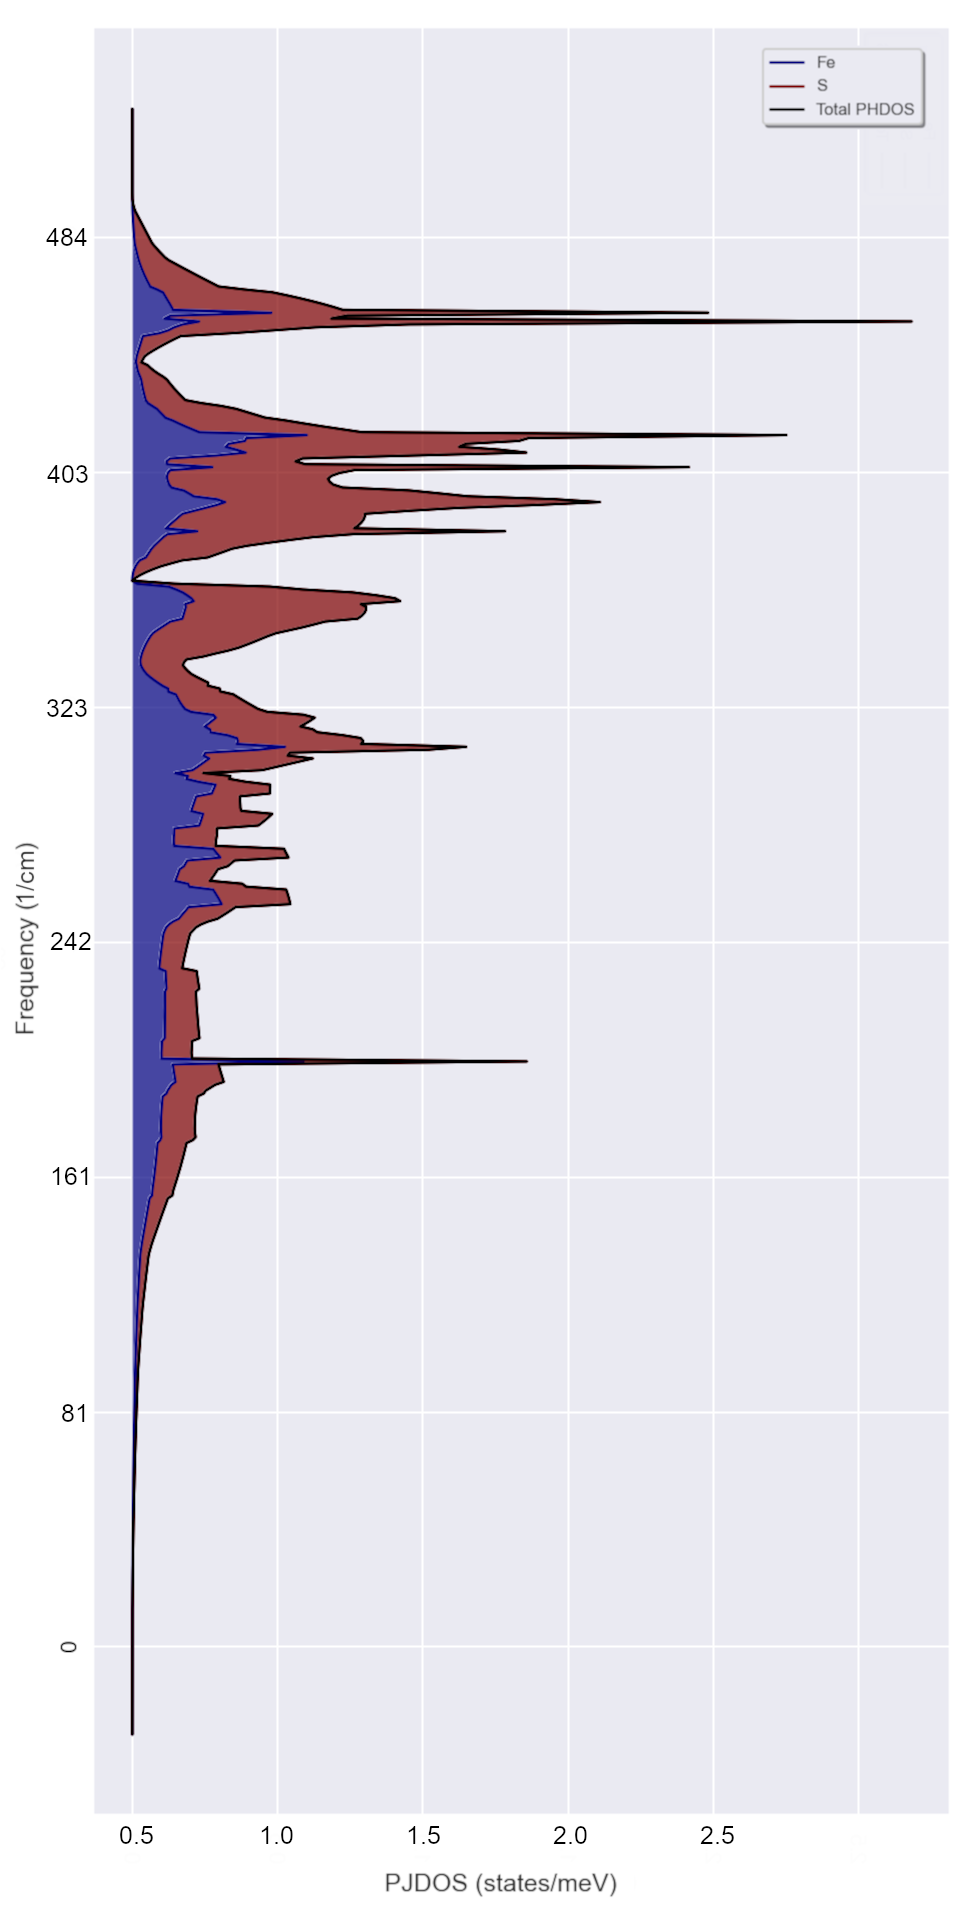
\includegraphics[width=\textwidth]{images/dos}
\caption{Computed phonon DOS plotted using \texttt{Abipy}}
\label{fig:phonondos1}
\end{subfigure}
\hfill
\begin{subfigure}[b]{0.35\textwidth}
\centering
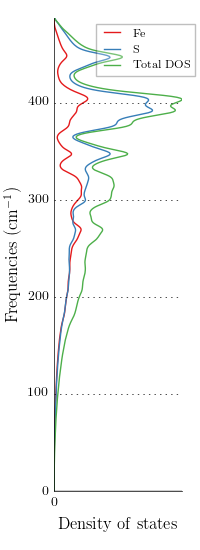
\includegraphics[width=\textwidth]{images/phonon_dos.png}
\caption{Phonon DOS provided by the Materials Project (\url{https://materialsproject.org/materials/mp-1522/})}
\label{fig:phonondos2}
\end{subfigure}
\caption{Comparison of the phonon DOS}
\label{fig:phonondos}
\end{figure}
\subsection{Dielectric tensor}
To compute the dielectric tensor of the material, a DFPT computation is performed using \texttt{Abinit}. In the input file (\autoref{Abi11}) three datasets are created : 
\begin{itemize}
\item The first one is used to generate the ground-state properties of the material, and the ground-state wavefunctions that will be used in the further computations.
\item The second dataset is used to compute the derivatives of the wavefunctions with respect to $k$ ($\frac{\text{d}}{\text{d}k}$ calculation).  
\item The third and last dataset is used to compute the response function under perturbations due to the electric field.
\end{itemize}
The obtained dielectric tensor is a diagonal $3\times 3$ tensor : 
\begin{equation}
\label{eqn:dielectricTens}\underline{\underline{\varepsilon}} = \left(\begin{array}{ccc}20.2021&0&0\\0&20.9923&0\\0&0&20.8858\end{array}\right)\end{equation}
\section{Results and macroscopic implications}
\subsection{Dielectric tensor}
From \autoref{eqn:dielectricTens}, the dielectric constant (relative permittivity) $\varepsilon_{r}$ of \ch{FeS2} can be computed :  
\begin{equation}
\label{eqn:dielectricCst}
\varepsilon_{r} = \dfrac{20.2021+20.9923+20.8858}{3} = 20.6934
\end{equation}
For comparison, the value provided by the Materials Project is $\varepsilon_r = 21.1311$. \\
The value of the electric susceptibility naturally follows \autoref{eqn:dielectricCst} : 
\begin{equation}
\label{eqn:electricSusc}
\chi = \varepsilon_r-1 = 19.693
\end{equation}
\subsection{Band structure and band gap}
As seen in \autoref{elecbs}, the band gap is indirect as the initial wavevector is $(0, 0.4, 0)$ and the final wavevector is $(0, 0, 0)$. The change of wavevector is represented on \autoref{fig:kbz}. The computed energy of the band gap is $0.8674$ eV (\autoref{tab:bg}). In a semiconducting material, the electrons of the last valence band are able to jump in the first conduction band by interacting with an incident photon and absorbing its energy. The energy of the interacting photons must be equal to that one of the bandgap in order to be absorbed by the electrons. It is thus possible to know the frequency of the absorbed light : 
\begin{equation}
\label{bgE}
E = h\nu = \hbar \omega
\end{equation}
with $h$ the Planck's constant and $\nu$ the frequency of the interacting photons. We get 
\begin{align}
\label{angfreq}
\nu &= \dfrac{0.8674\times 1.60218\times 10^{-19}}{6.62607\times 10^{-34}}\text{ Hz}\\
&= 2.09737\times 10^{14}\text{\space Hz}\\
&=209.737 \texttt{\space THz}
\end{align}
It corresponds to IR-B photons \cite{irb}.
\begin{figure}
\centering
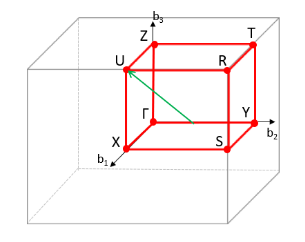
\includegraphics[width=0.3\textwidth]{images/kbz}
\caption{Brillouin zone for a simple orthorhombic lattice. The change of wavevector through the band gap is represented by the green arrow.}
\label{fig:kbz}
\end{figure}

Although the material studied here is not candidate for future photovoltaic applications, its cubic polymorph, \textit{pyrite}, is. The band gap of the latter material is also indirect \cite{MaterialsProjectPyrite}. It means that in order to generate a free electron-hole pair, one electron of the last valence band will have to interact with an incident photon and a phonon of the crystal lattice. This is why the phonon dipsersion and density of states can be interesting. Furthermore, it can be used to assess the thermal management of the material when exposed to light. 
In general, that kind of event (interaction with a photon and a phonon at the same time) is far more uncommon than for a direct bandgap, and the photons will penetrate deeper in the material before being absorbed. So in order to absorbed as much light as possible, the layer of material will have to be sufficiently thick \cite{gaps}.
\subsection{Optics}
When designing a photovoltaic cell, the material is wanted to have a maximum absorption and a minimum reflectivity, in order to mobilize as much incident light as possible. It implies that the refractive index must be as low as possible. Moreover, the photons have to be absorbed near the $pn$-junction to generate carriers. It is thus interesting to investigate the frequency dependent properties of the material, as for example the complex frequency dependent dielectric tensor $\tilde{\varepsilon}_r(\omega)$. Those quantities can then bu used to know the frequency dependent refractive index $n(\omega)$, and extinction coefficient $\kappa(\omega)$ as 
\begin{align}
\tilde{\varepsilon}_r(\omega) &= \tilde{n}^2(\omega)\\
&= (n(\omega)+j\kappa(\omega))^2
\end{align}
This can be done using the \texttt{Optic} module of \texttt{Abinit}. However, as those kind of computations can be very time-consuming, it should be done with the material of interest, \textit{pyrite} in this case. The absorption of the material in the visible range of light can be analyzed, and the effect of various modifications of the material can be studied (for example doping). 
\section{Conclusion}
Marcassite is an orthorhombic polymorph of pyrite, of chemical formula $\ch{FeS2}$. Several computations have been performed using \texttt{Abinit} to assess (part of) its optical properties : DFT calculations to get the electronic bandstructure and density of state, and response function calculations to get data about the phonons in the material (phonon dispersion and density of stats) and its dielectric tensor. The results have been compared with the Materials Project and good agreement between the two sources has been showed in general. The similarities between marcassite and pyrite allows to expect some of properties of the latter crystal, and predict some of the properties to take into account to make efficient pyrite-based solar cells.

No need to say that this report could have been far more complete, even if some of the obtained results are satisfactory. Indeed, more convergence studies have to be done in order to ensure that the parameters ruling the different computations allow reliable results, even if they were chosen as wisely as possible during the writing of these lines. Furthermore, more optical properties of the crystal could be computed, using the \texttt{Optic} module. However, the convergence studies and the SCF calculations needed to run the \texttt{Optic} computations are very time-consuming. 

\hspace{1cm}\\
This project allowed me to grasp all of the potential of the \texttt{Abinit} package and its working principle. Besides using the theoretical concepts seen during the classes, I could understand the specificities of intensive computing at a larger scale. I would like to thank Bogdan and Alexandre for their support during the project, their advices and the help they provided during the semester. 
\newpage
\phantom{\cite{fox}}
\phantom{\cite{azzamBashara}}
\bibliographystyle{IEEEtran}
\bibliography{biblio}
\newpage
\appendix
\section{Convergence of the total energy per atom as a function of \texttt{ecut}}
\label{Abi1}
Name of the input file : \texttt{1522\_3\_ecutConv.abi}
\begin{center}
\begin{tabular}{lll}
\texttt{acell} & \texttt{3.390} \texttt{4.438} \texttt{5.411} \texttt{Angstr} & \\
\texttt{ntypat} & \texttt{2} &\\
\texttt{znucl} & \texttt{26 16}& \\
\texttt{natom} & \texttt{6} & \\
\texttt{typat} & \texttt{1 1 2 2 2 2}&\\
\texttt{xred} & \texttt{0\space\space\space\space\space\space 0\space\space\space\space\space\space 0} & \\
& \texttt{0.5\space\space\space\space 0.5\space\space\space\space0.5} & \\
& \texttt{0\space\space\space\space\space\space 0.206\space\space 0.3753} & \\
& \texttt{0\space\space\space\space\space\space 0.794\space\space 0.6247} & \\
& \texttt{0.5\space\space\space\space 0.294\space\space 0.8753} & \\
& \texttt{0.5\space\space\space\space 0.706\space\space 0.1247} & \\
&&\\
\texttt{pseudos} & \multicolumn{2}{l}{\texttt{"Fe.psp8,S.psp8"}}\\
&&\\
\multicolumn{3}{l}{\texttt{\# parameters of the SCF procedure : }}\\
\texttt{nstep} & \texttt{100} &\texttt{\# maximal number of SCF cycles}\\
\texttt{toldfe} & \texttt{1.0d-10} &\texttt{\# SCF procedure will stop when the difference of total}\\
&&\texttt{\#\space\space\space\space energy between two iterations will be lower than}\\
&&\texttt{\#\space\space\space\space toldfe Hartree}\\
\texttt{diemac} &\texttt{24.0} & \texttt{\# preconditioning of the SCF procedure.}\\
&&\\
\multicolumn{3}{l}{\texttt{\# parameters for generating the k-points grids : }}\\
\texttt{kptopt} & \texttt{1} &\\
\texttt{ngkpt} & \texttt{3 3 4}&\\
\texttt{nshiftk} &\texttt{1}&\\
\texttt{shiftk} &\texttt{0.5 0.5 0.5}&\\
&&\\
\texttt{ndtset} &\texttt{50}&\\
\texttt{ecut:}&\texttt{10}&\\
\texttt{ecut+}&\texttt{1}&\\ 
\end{tabular}
\end{center} 
\newpage
\section{Convergence of the total energy per atom as a function of \texttt{ngkpt}}
\label{Abi2}
Name of the input file : \texttt{1522\_4\_nkpConv.abi}
\begin{center}
\begin{tabular}{lll}
\texttt{acell} & \texttt{3.390} \texttt{4.438} \texttt{5.411} \texttt{Angstr} & \\
\texttt{ntypat} & \texttt{2} &\\
\texttt{znucl} & \texttt{26 16}& \\
\texttt{natom} & \texttt{6} & \\
\texttt{typat} & \texttt{1 1 2 2 2 2}&\\
\texttt{xred} & \texttt{0\space\space\space\space\space\space 0\space\space\space\space\space\space 0} & \\
& \texttt{0.5\space\space\space\space 0.5\space\space\space\space0.5} & \\
& \texttt{0\space\space\space\space\space\space 0.206\space\space 0.3753} & \\
& \texttt{0\space\space\space\space\space\space 0.794\space\space 0.6247} & \\
& \texttt{0.5\space\space\space\space 0.294\space\space 0.8753} & \\
& \texttt{0.5\space\space\space\space 0.706\space\space 0.1247} & \\
\texttt{ecut} &\texttt{40}&\texttt{\# the converged value for ecut} \\
&&\\
\texttt{pseudos} & \multicolumn{2}{l}{\texttt{"/Fe.psp8,S.psp8"}}\\
&&\\
\multicolumn{3}{l}{\texttt{\# parameters of the SCF procedure : }}\\
\texttt{nstep} & \texttt{100} &\texttt{\# maximal number of SCF cycles}\\
\texttt{toldfe} & \texttt{1.0d-10} &\texttt{\# SCF procedure will stop when the difference of total}\\
&&\texttt{\#\space\space\space\space energy between two iterations will be lower than}\\
&&\texttt{\#\space\space\space\space toldfe Hartree}\\
\texttt{diemac} &\texttt{24.0} & \texttt{\# preconditioning of the SCF procedure.}\\
&&\\
\multicolumn{3}{l}{\texttt{\# parameters for generating the k-points grids : }}\\
\texttt{getwfk} & \texttt{-1}&\\
\texttt{kptopt} & \texttt{1} &\\
\texttt{ndtset} & \texttt{6}&\\
\texttt{ngkpt1} & \texttt{2 2 2}&\\
\texttt{ngkpt2} & \texttt{2 2 3}&\\
\texttt{ngkpt3} & \texttt{3 3 3}&\\
\texttt{ngkpt4} & \texttt{3 3 4}&\\
\texttt{ngkpt5} & \texttt{4 4 4}&\\
\texttt{ngkpt6} & \texttt{4 4 5}&\\
\texttt{nshiftk} &\texttt{1}&\\
\texttt{shiftk} &\texttt{0.5 0.5 0.5}&
\end{tabular}
\end{center} 
\newpage
\section{Convergence of the lattice scale parameters as a function of \texttt{ecut}}
\label{Abi3}
Name of the input file : \texttt{1522\_6\_acellEcutConv.abi}
\begin{center}
\begin{tabular}{lll}
\texttt{acell} & \texttt{3.390} \texttt{4.438} \texttt{5.411} \texttt{Angstr} & \\
\texttt{ntypat} & \texttt{2} &\\
\texttt{znucl} & \texttt{26 16}& \\
\texttt{natom} & \texttt{6} & \\
\texttt{typat} & \texttt{1 1 2 2 2 2}&\\
\texttt{xred} & \texttt{0\space\space\space\space\space\space 0\space\space\space\space\space\space 0} & \\
& \texttt{0.5\space\space\space\space 0.5\space\space\space\space0.5} & \\
& \texttt{0\space\space\space\space\space\space 0.206\space\space 0.3753} & \\
& \texttt{0\space\space\space\space\space\space 0.794\space\space 0.6247} & \\
& \texttt{0.5\space\space\space\space 0.294\space\space 0.8753} & \\
& \texttt{0.5\space\space\space\space 0.706\space\space 0.1247} & \\
&&\\
\texttt{ndtset} &\texttt{16}&\\
\texttt{ecut:} &\texttt{20}&\\
\texttt{ecut+} &\texttt{2}&\\
&&\\
\texttt{pseudos} & \multicolumn{2}{l}{\texttt{"/Fe.psp8,S.psp8"}}\\
&&\\
\multicolumn{3}{l}{\texttt{\# parameters of the SCF procedure : }}\\
\texttt{nstep} & \texttt{100} &\texttt{\# maximal number of SCF cycles}\\
\texttt{toldff} & \texttt{1.0d-6} &\texttt{\# SCF procedure will stop when the difference of total}\\
&&\texttt{\#\space\space\space\space energy between two iterations will be lower than}\\
&&\texttt{\#\space\space\space\space toldfe Hartree}\\
\texttt{diemac} &\texttt{24.0} & \texttt{\# preconditioning of the SCF procedure.}\\
&&\\
\texttt{ionmov} & \texttt{2} &\\
\texttt{optcell} &\texttt{1}&\\
\texttt{dilatmx} &\texttt{1.05}&\\
\texttt{ecutsm} &\texttt{0.5}&\\
\texttt{kptopt}&\texttt{1}&\\
\texttt{ngkpt}&\texttt{3 3 3}&\\
\texttt{nshiftk}&\texttt{1}&\\
\texttt{shiftk}&\texttt{0.5 0.5 0.5}&\\
\texttt{getwfk}&\texttt{-1}&\\
\end{tabular}
\end{center} 
\newpage
\section{Convergence of the lattice scale parameters as a function of \texttt{ngkpt}}
\label{Abi4}
Name of the input file : \texttt{1522\_3\_acellNgkptConv.abi}
\begin{center}
\begin{tabular}{lll}
\texttt{acell} & \texttt{3.390} \texttt{4.438} \texttt{5.411} \texttt{Angstr} & \\
\texttt{ntypat} & \texttt{2} &\\
\texttt{znucl} & \texttt{26 16}& \\
\texttt{natom} & \texttt{6} & \\
\texttt{typat} & \texttt{1 1 2 2 2 2}&\\
\texttt{xred} & \texttt{0\space\space\space\space\space\space 0\space\space\space\space\space\space 0} & \\
& \texttt{0.5\space\space\space\space 0.5\space\space\space\space0.5} & \\
& \texttt{0\space\space\space\space\space\space 0.206\space\space 0.3753} & \\
& \texttt{0\space\space\space\space\space\space 0.794\space\space 0.6247} & \\
& \texttt{0.5\space\space\space\space 0.294\space\space 0.8753} & \\
& \texttt{0.5\space\space\space\space 0.706\space\space 0.1247} & \\
&&\\
\texttt{ndtset} &\texttt{6}&\\
\texttt{ngkpt1} &\texttt{2 2 2}&\\
\texttt{ngkpt2} &\texttt{2 2 3}&\\
\texttt{ngkpt3} &\texttt{3 3 3}&\\
\texttt{ngkpt4} &\texttt{3 3 4}&\\
\texttt{ngkpt5} &\texttt{4 4 4}&\\
\texttt{ngkpt6} &\texttt{4 4 5}&\\
&&\\
\texttt{ecut} &\texttt{40}&\\
\texttt{pseudos} & \multicolumn{2}{l}{\texttt{"/Fe.psp8,S.psp8"}}\\
&&\\
\multicolumn{3}{l}{\texttt{\# parameters of the SCF procedure : }}\\
\texttt{nstep} & \texttt{100} &\texttt{\# maximal number of SCF cycles}\\
\texttt{toldff} & \texttt{1.0d-6} &\texttt{\# SCF procedure will stop when the difference of total}\\
&&\texttt{\#\space\space\space\space energy between two iterations will be lower than}\\
&&\texttt{\#\space\space\space\space toldfe Hartree}\\
\texttt{diemac} &\texttt{24.0} & \texttt{\# preconditioning of the SCF procedure.}\\
&&\\
\texttt{ionmov} & \texttt{2} &\\
\texttt{optcell} &\texttt{1}&\\
\texttt{dilatmx} &\texttt{1.05}&\\
\texttt{ecutsm} &\texttt{0.5}&\\
\texttt{nshiftk}&\texttt{1}&\\
\texttt{shiftk}&\texttt{0.5 0.5 0.5}&\\
\texttt{getwfk}&\texttt{-1}&\\
\end{tabular}
\end{center} 
\newpage
\section{Band structure : $k$-path generation using Absitruct (Abipy)}
\label{Abi5}
Command used : \texttt{abistruct.py kpath input.abi}\\[0.5cm]
Input file : \texttt{input.abi} :\\
\begin{tabular}{lll}
\texttt{acell} &\texttt{3.315 4.3398 5.2913 Angstr}&\texttt{\# the converged values}\\
\texttt{ntypat}&\texttt{2}\\
\texttt{znucl}&\texttt{26 16}\\
\texttt{natom}&\texttt{6}\\
\texttt{typat}&\texttt{1 1 2 2 2 2}\\
\texttt{xred} &&\texttt{\# the converged values}\\
&\texttt{0\space\space\space0\space\space\space\space\space\space\space0}&\\
&\texttt{0.5 0.5 \space\space\space\space0.5}&\\
&\texttt{0\space\space\space0.20809 0.37374}&\\
&\texttt{0\space\space\space0.79191 0.62626}&\\
&\texttt{0.5 0.29191 0.87374}&\\
&\texttt{0.5 0.70809 0.12626}&\\
\texttt{pseudos} & \multicolumn{2}{l}{\texttt{"/Fe.psp8,S.psp8"}}\\
\texttt{nstep} &\texttt{100}&\\
\texttt{toldfe} &\texttt{1.0d-10}&\\
\texttt{diemac} &\texttt{24.0}&\\
\texttt{kptopt} &\texttt{1}&\\
\texttt{ngkpt} &\texttt{3 3 3}&\\
\texttt{nshiftk} &\texttt{1}&\\
\texttt{shiftk} &\texttt{0.5 0.5 0.5}&\\
\texttt{getwfk} &\texttt{-1}&\\
\end{tabular}
\newpage
Output :\\
\begin{tabular}{lll}
\multicolumn{3}{l}{\texttt{\# Abinit structure}}\\
\texttt{natom}&\texttt{6}\\
\texttt{ntypat}&\texttt{2}\\
\texttt{typat}&\texttt{1 1 2 2 2 2}\\
\texttt{znucl}&\texttt{26 16}\\
\texttt{xred} &&\texttt{\# the converged values}\\
&\texttt{0\space\space\space0\space\space\space\space\space\space\space0}&\\
&\texttt{0.5 0.5 \space\space\space\space0.5}&\\
&\texttt{0\space\space\space0.20809 0.37374}&\\
&\texttt{0\space\space\space0.79191 0.62626}&\\
&\texttt{0.5 0.29191 0.87374}&\\
&\texttt{0.5 0.70809 0.12626}&\\
\texttt{acell}&\texttt{1.0 1.0 1.0}&\\
\texttt{rprim}&&\\
&\texttt{6.2644421031 0.0000000000 0.0000000000}&\\
&\texttt{0.0000000000 8.2010334357 0.0000000000}&\\
&\texttt{0.0000000000 0.0000000000 9.9991078432}&\\
\multicolumn{3}{l}{\texttt{\# tolwfr 1e-20 iscf -2 \# NSCF run}}\\
\multicolumn{3}{l}{\texttt{\# To read previous DEN file, use: getden -1 or specify filename via getden\_path "out\_DEN"
}}\\
\multicolumn{3}{l}{\texttt{\textsc{\# K-path in reduced coordinates:
}}}\\
\texttt{ndivsm} & \texttt{10}&\\
\texttt{kptopt} &\texttt{-15}&\\
\texttt{kptbounds}&&\\
&\texttt{+0.00000 +0.00000 +0.00000}&\texttt{\# \$\textbackslash Gamma\$}\\
&\texttt{+0.50000  +0.00000  +0.00000}&\texttt{\# X}\\
&\texttt{+0.50000  +0.50000  +0.00000}&\texttt{\# S}\\
&\texttt{+0.00000  +0.50000  +0.00000}&\texttt{\# Y}\\
&\texttt{+0.00000  +0.00000  +0.00000}&\texttt{\# \$\textbackslash Gamma\$}\\
&\texttt{+0.00000  +0.00000  +0.50000}&\texttt{\# Z}\\
&\texttt{+0.50000  +0.00000  +0.50000}&\texttt{\# U}\\
&\texttt{+0.50000  +0.50000  +0.50000}&\texttt{\# R}\\
&\texttt{+0.00000  +0.50000  +0.50000}&\texttt{\# T}\\
&\texttt{+0.00000  +0.00000  +0.50000}&\texttt{\# Z}\\
&\texttt{+0.00000  +0.50000  +0.00000}&\texttt{\# Y}\\
&\texttt{+0.00000  +0.50000  +0.50000}&\texttt{\# T}\\
&\texttt{+0.50000  +0.00000  +0.50000}&\texttt{\# U}\\
&\texttt{+0.50000  +0.00000  +0.00000}&\texttt{\# X}\\
&\texttt{+0.50000  +0.50000  +0.00000}&\texttt{\# S}\\
&\texttt{+0.50000  +0.50000  +0.50000}&\texttt{\# R}\\
\end{tabular}
\newpage
\section{Band structure computation}
\label{Abi6}
\begin{center}
\begin{tabular}{lll}
\texttt{ndtset}&\texttt{2}&\\
\texttt{natom} &\texttt{6}&\\
\texttt{typas} &\texttt{1 1 2 2 2 2}&\\
\texttt{xred} &&\\
&\texttt{0.0000000000    0.0000000000    0.0000000000}&\\
&\texttt{0.5000000000    0.5000000000    0.5000000000}&\\
&\texttt{0.0000000000    0.2080900000    0.3737400000}&\\
&\texttt{0.0000000000    0.7919100000    0.6262600000}&\\
&\texttt{0.5000000000    0.2919100000    0.8737400000}&\\
&\texttt{0.5000000000    0.7080900000    0.1262600000}&\\
\texttt{ecut} &\texttt{40.0}&\texttt{\# converged value}\\
\multicolumn{3}{l}{\texttt{\# definition of the SCF procedure}}\\
\texttt{nstep}&\texttt{100}&\\
\texttt{diemac}&\texttt{24.0}&\\
\multicolumn{3}{l}{\texttt{\# first dataset : SCF density computation}}\\
\texttt{kptopt1}&\texttt{1}&\\
\texttt{nshiftk1}&\texttt{1}&\\
\texttt{shiftk1}&\texttt{0.5 0.5 0.5}&\\
\texttt{ngkpt1}&\texttt{3 3 3}&\texttt{\# converged value}\\
\texttt{prtden1}&\texttt{1}&\\
\texttt{toldfe1}&\texttt{1.0d-10}&\\
\multicolumn{3}{l}{\texttt{\# second dataset : band structure computation}}\\
\texttt{iscf2}&\texttt{-2}&\\
\texttt{getden2}&\texttt{-1}&\\
\texttt{kptopt2}&\texttt{-15}&\texttt{\# number of k-segments}\\
\texttt{nband2}&\texttt{35}&\texttt{\# numbe rof bands}\\
\texttt{nbdbuf}&\texttt{-2}&\\
\texttt{ndivsm2}&\texttt{30}&\\
\texttt{kptbounds}&&\\
&\texttt{+0.00000 +0.00000 +0.00000}&\texttt{\# \$\textbackslash Gamma\$}\\
&\texttt{+0.50000  +0.00000  +0.00000}&\texttt{\# X}\\
&\texttt{+0.50000  +0.50000  +0.00000}&\texttt{\# S}\\
&\texttt{+0.00000  +0.50000  +0.00000}&\texttt{\# Y}\\
&\texttt{+0.00000  +0.00000  +0.00000}&\texttt{\# \$\textbackslash Gamma\$}\\
&\texttt{+0.00000  +0.00000  +0.50000}&\texttt{\# Z}\\
&\texttt{+0.50000  +0.00000  +0.50000}&\texttt{\# U}\\
&\texttt{+0.50000  +0.50000  +0.50000}&\texttt{\# R}\\
&\texttt{+0.00000  +0.50000  +0.50000}&\texttt{\# T}\\
&\texttt{+0.00000  +0.00000  +0.50000}&\texttt{\# Z}\\
&\texttt{+0.00000  +0.50000  +0.00000}&\texttt{\# Y}\\
&\texttt{+0.00000  +0.50000  +0.50000}&\texttt{\# T}\\
&\texttt{+0.50000  +0.00000  +0.50000}&\texttt{\# U}\\
&\texttt{+0.50000  +0.00000  +0.00000}&\texttt{\# X}\\
&\texttt{+0.50000  +0.50000  +0.00000}&\texttt{\# S}\\
&\texttt{+0.50000  +0.50000  +0.50000}&\texttt{\# R}\\
\texttt{tolwfr2}&\texttt{1.0d-12}&\\
\texttt{enunit2}&\texttt{1}&\texttt{\# to get the energies in eV}\\
\end{tabular}
\end{center}
\newpage
\section{Band structure : Materials Project}
\label{Abi7}
\begin{figure}[h]
\centering
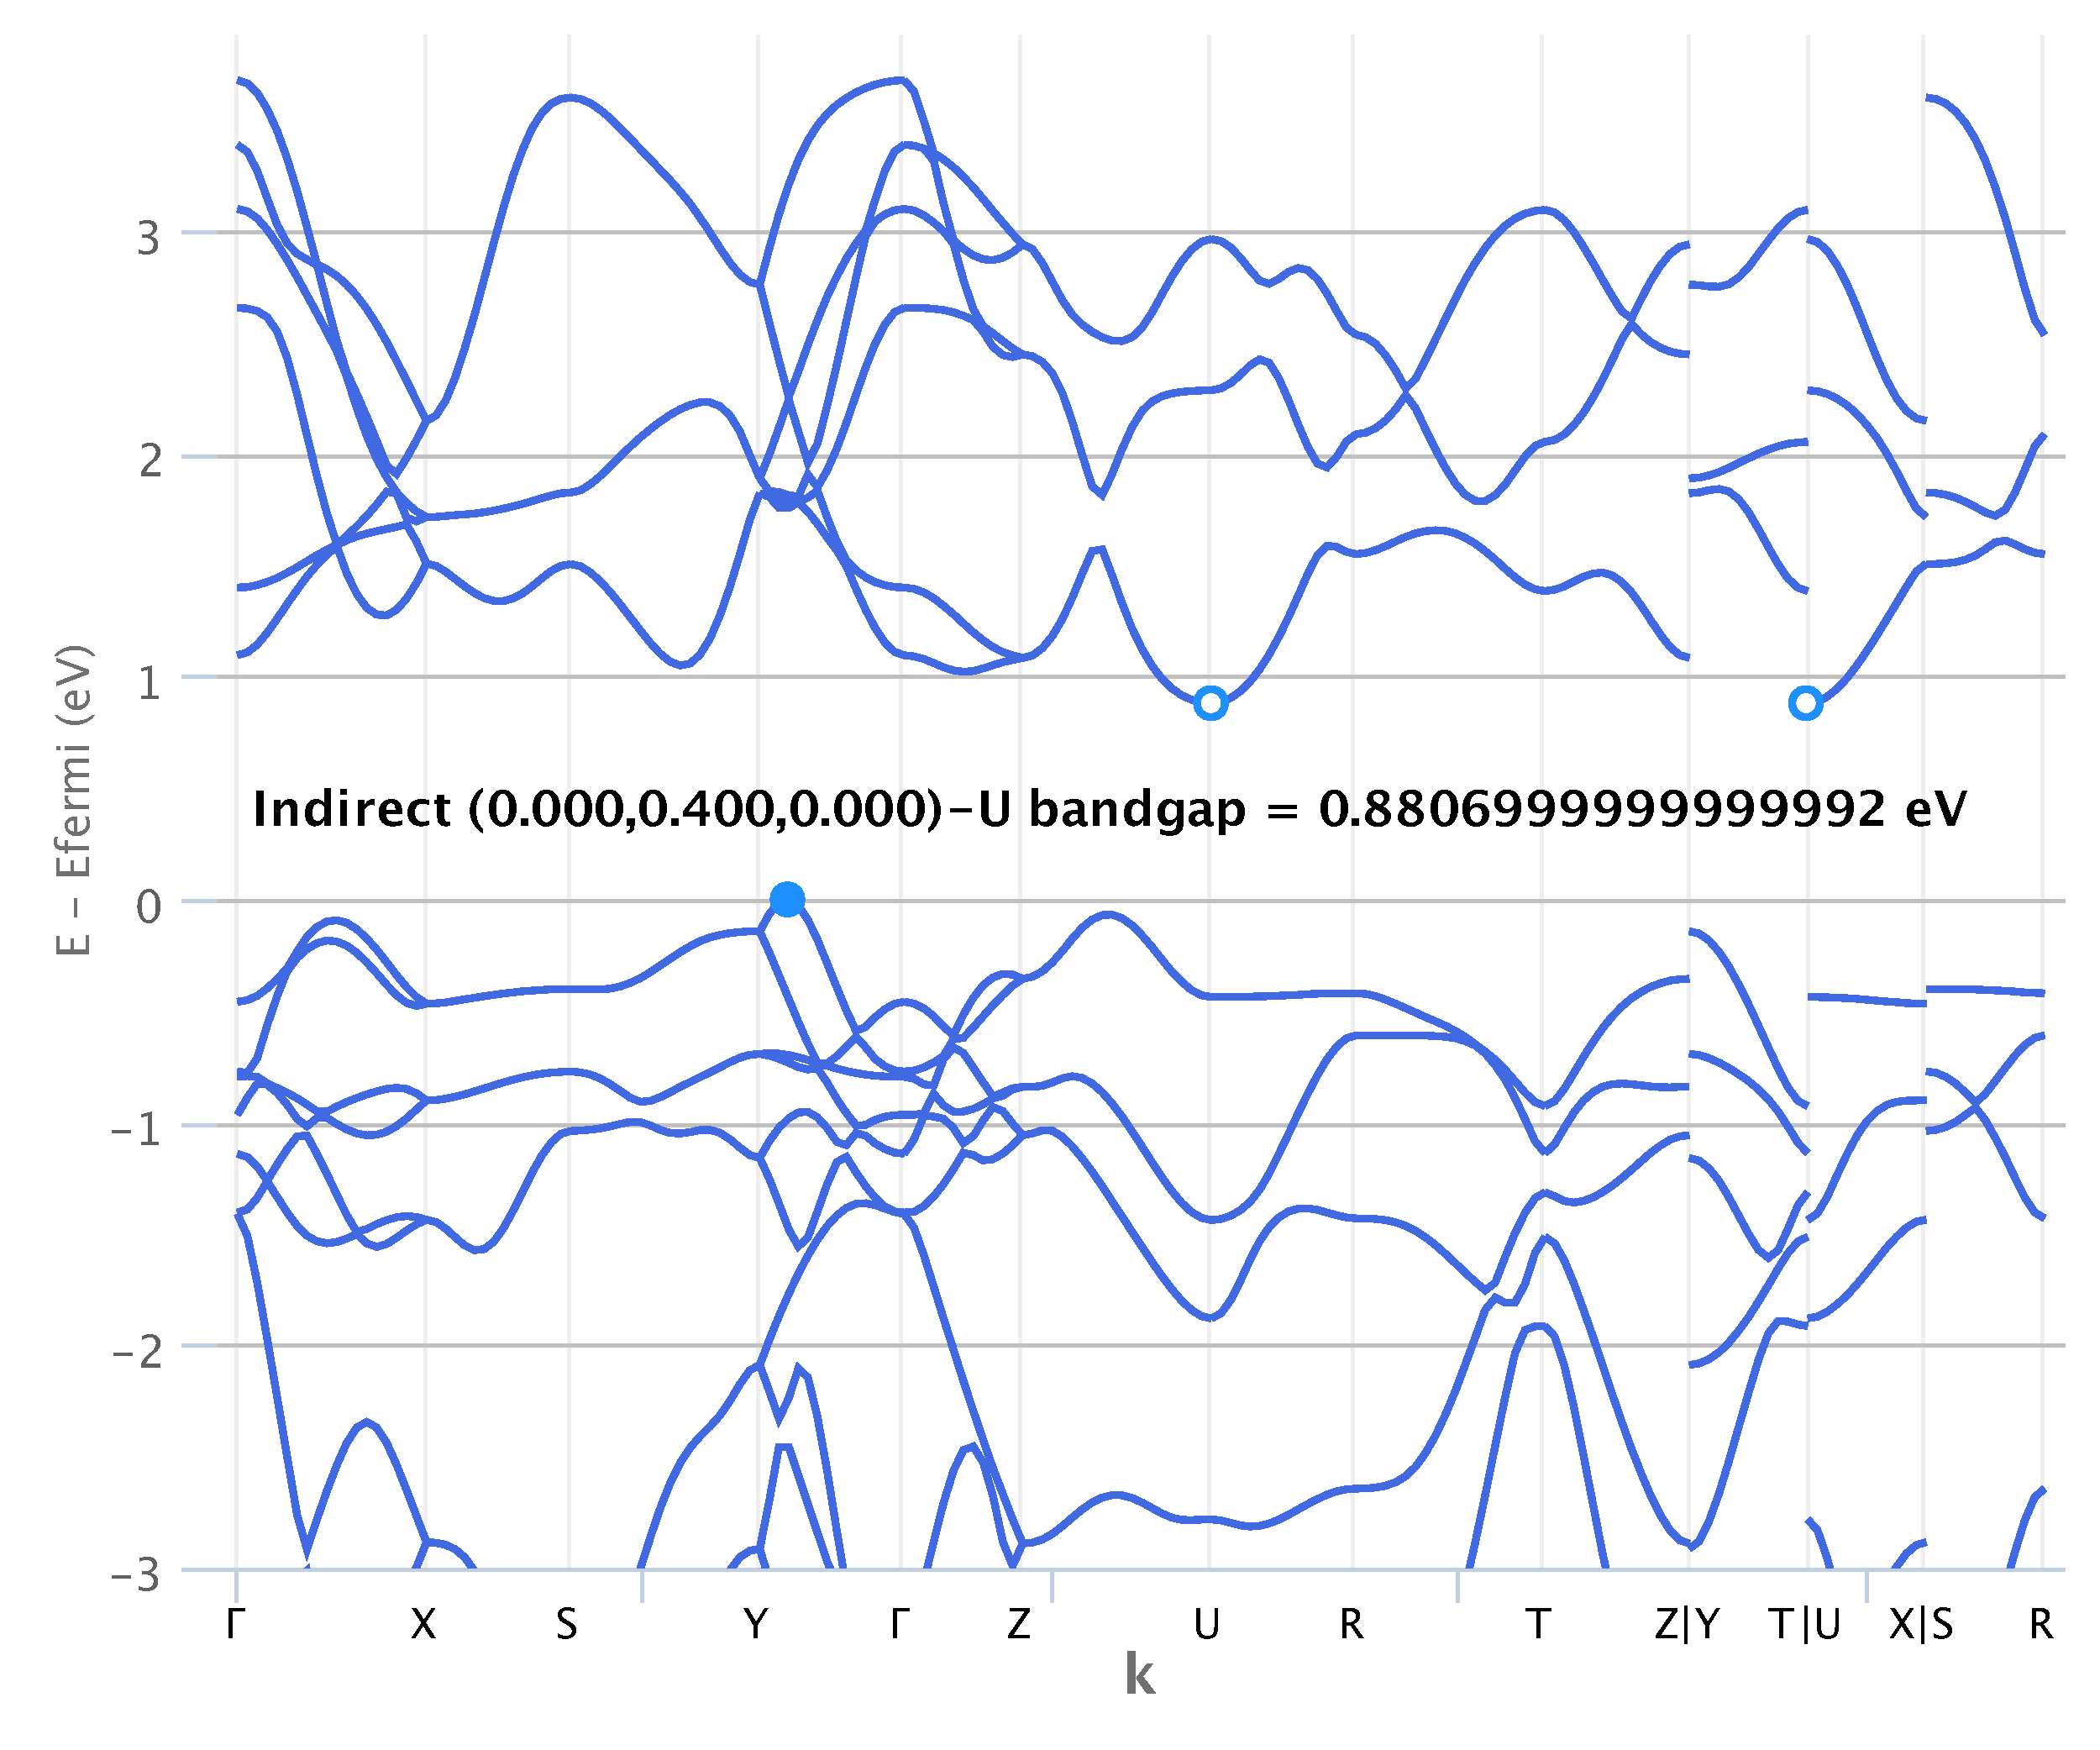
\includegraphics[width=\textwidth]{images/chart.pdf}
\caption{Band structure of orthorhombic \ch{FeS2} provided by the Materials Project}
\end{figure}
\newpage
\section{Electronic density of states}
\label{Abi8}
\begin{center}
\begin{tabular}{lll}
\multicolumn{3}{l}{\texttt{\# computation of the electronic DOS}}\\
\texttt{ndtset} & \texttt{2}&\\
\multicolumn{3}{l}{\texttt{\# definition of the unit cell}}\\
\texttt{acell} & \texttt{1.0 1.0 1.0}&\\
\texttt{rprim}&&\\
&\texttt{6.2644421031    0.0000000000    0.0000000000}&\\
&\texttt{0.0000000000    8.2010334357    0.0000000000}&\\
&\texttt{0.0000000000    0.0000000000    9.9991078432}&\\
\multicolumn{3}{l}{\texttt{\# definition of the atoms types}}\\
\texttt{ntypat}&\texttt{2}&\\
\texttt{znucl}&\texttt{26 16}&\\
\texttt{pseudos}&\texttt{"Fe.psp8,S.psp8"}&\\
\multicolumn{3}{l}{\texttt{\# definition of the atoms}}\\
\texttt{natom}&\texttt{6}&\\
\texttt{typat}&\texttt{1 1 2 2 2 2}&\\
\texttt{xred} &&\\
&\texttt{0.0000000000    0.0000000000    0.0000000000}&\\
&\texttt{0.5000000000    0.5000000000    0.5000000000}&\\
&\texttt{0.0000000000    0.2080900000    0.3737400000}&\\
&\texttt{0.0000000000    0.7919100000    0.6262600000}&\\
&\texttt{0.5000000000    0.2919100000    0.8737400000}&\\
&\texttt{0.5000000000    0.7080900000    0.1262600000}&\\
\texttt{ecut} &\texttt{40.0}&\texttt{\# converged value}\\
\multicolumn{3}{l}{\texttt{\# first dataset : SCF density computation}}\\
\multicolumn{3}{l}{\texttt{\# definition of the SCF procedure}}\\
\texttt{toldfe1}&\texttt{1.0d-10}&\\
\texttt{nstep}&\texttt{100}&\\
\texttt{diemac}&\texttt{24.0}&\\
\multicolumn{3}{l}{\texttt{\# Brillouin zone sampling}}\\
\texttt{kptopt1}&\texttt{1}&\\
\texttt{nshiftk1}&\texttt{1}&\\
\texttt{shiftk1}&\texttt{0 0 0}&\texttt{\# use of a non-shifted k-grid}\\
\texttt{ngkpt1}&\texttt{8 8 8}&\texttt{\# higher than the converged value to}\\
&&\texttt{\# obtain a good resolution in the}\\
&&\texttt{\# DOS plot}\\
\texttt{prtden1}&\texttt{1}&\\
\multicolumn{3}{l}{\texttt{\# second dataset : DOS computation}}\\
\texttt{prtdos2}&\texttt{2}&\texttt{\# computing the DOS using the}\\
&&\texttt{\# wtetrahedron method}\\
\texttt{getden2}&\texttt{-1}&\\
\texttt{iscf2}&\texttt{-3}&\\
\texttt{tolwfr2}&\texttt{1.0d-12}&\\
\texttt{dosdeltae2}&\texttt{5.0d-5}&\\
\end{tabular}
\end{center}
\newpage
\section{Phonons : Generation of a list of $q$-points}
\label{Abi9}
\begin{center}
\begin{tabular}{lll}
\multicolumn{3}{l}{\texttt{\# Pnnm [58] FeS2 : computation of the q points}}\\
\texttt{ngkpt} & \texttt{3 3 3} & \\
\texttt{nshiftk} & \texttt{1} & \\
\texttt{shiftk} & \texttt{0 0 0} & \\
\multicolumn{3}{l}{\texttt{\# dummy SCF procedure}}\\
\texttt{nstep} & \texttt{1} & \\
\texttt{nline} & \texttt{1} & \\
\texttt{diemac} &\texttt{24.0}\\
\multicolumn{3}{l}{\texttt{\# common input variables}}\\
\texttt{acell} & \texttt{1.0 1.0 1.0} & \\
\texttt{rprim}&&\\
&\texttt{6.2644421031    0.0000000000    0.0000000000}&\\
&\texttt{0.0000000000    8.2010334357    0.0000000000}&\\
&\texttt{0.0000000000    0.0000000000    9.9991078432}&\\
\texttt{ntypat} & \texttt{2} & \\
\texttt{znucl} & \texttt{26 16} & \\
\texttt{pseudos}&\texttt{"Fe.psp8,S.psp8"}&\\
\texttt{natom}&\texttt{6}&\\
\texttt{typat}&\texttt{1 1 2 2 2 2}&\\
\texttt{xred} &&\\
&\texttt{0.0000000000    0.0000000000    0.0000000000}&\\
&\texttt{0.5000000000    0.5000000000    0.5000000000}&\\
&\texttt{0.0000000000    0.2080900000    0.3737400000}&\\
&\texttt{0.0000000000    0.7919100000    0.6262600000}&\\
&\texttt{0.5000000000    0.2919100000    0.8737400000}&\\
&\texttt{0.5000000000    0.7080900000    0.1262600000}&\\
\texttt{ecut} &\texttt{40.0}&\texttt{\# converged value}\\
\texttt{nband} & \texttt{35} &\\
\texttt{tolvrs} &\texttt{1.0d-18}&\texttt{\# dummy variable as there is only one}\\
&&\texttt{\# step in the SCF procedure}
\end{tabular}
\end{center}
\newpage
\section{Phonons : Generation of the derivative databases}
\label{Abi10}
\begin{center}
\begin{tabular}{lll}
\texttt{ndtset} &\texttt{10}&\\
\multicolumn{3}{l}{\texttt{\# dataset 1 : GS self-consistent computation}}\\
\texttt{getwfk1} &\texttt{0}&\\
\texttt{kptopt1} &\texttt{1}&\\
\texttt{nqpt1} &\texttt{0}&\\
\texttt{tolvrs1} &\texttt{1.0d-18}&\\
\texttt{rfphon1} &\texttt{0}&\\
\multicolumn{3}{l}{\texttt{\# Q vectors for all datasets}}\\
\texttt{nqpt} &\texttt{1}&\\
\texttt{qpt2} &\texttt{0.00000000E+00  0.00000000E+00  0.00000000E+00}&\\
\texttt{qpt3} &\texttt{0.00000000E+00  0.00000000E+00  0.00000000E+00}&\\
\texttt{qpt4} &\texttt{3.33333333E-01  0.00000000E+00  0.00000000E+00}&\\
\texttt{qpt5} &\texttt{0.00000000E+00  3.33333333E-01  0.00000000E+00}&\\
\texttt{qpt6} &\texttt{3.33333333E-01  3.33333333E-01  0.00000000E+00}&\\
\texttt{qpt7} &\texttt{0.00000000E+00  0.00000000E+00  3.33333333E-01}&\\
\texttt{qpt8} &\texttt{3.33333333E-01  0.00000000E+00  3.33333333E-01}&\\
\texttt{qpt9} &\texttt{0.00000000E+00  3.33333333E-01  3.33333333E-01}&\\
\texttt{qpt10} &\texttt{3.33333333E-01  3.33333333E-01  3.33333333E-01}&\\
\multicolumn{3}{l}{\texttt{\# dataset 2 : response function calculation of d/dk wave function}}\\
\texttt{iscf2} & \texttt{-3} & \\
\texttt{kptopt2} & \texttt{2} & \\
\texttt{rfphon2} & \texttt{0} & \\
\texttt{rfelfd2} & \texttt{2} & \\
\texttt{tolwfr2} & \texttt{1.0d-22} & \\
\multicolumn{3}{l}{\texttt{\# dataset 3 : response function calculation at Q=0 phonons and electric field perturbation}}\\
\texttt{getddk3} & \texttt{2} & \\
\texttt{kptopt3} & \texttt{2} & \\
\texttt{rfelfd3} & \texttt{3} & \\
\end{tabular}
\end{center}
\begin{center}
\begin{tabular}{lll}
\multicolumn{3}{l}{\texttt{\# datasets 4-10 : finite-wave-vector phonon calculations (default for all datasets)}}\\
\texttt{getwfk} & \texttt{1} & \\
\texttt{kptopt} & \texttt{3} & \\
\texttt{rfphon} & \texttt{1} & \\
\texttt{rfatpol} & \texttt{1 6} & \\
\texttt{rfdir} & \texttt{1 1 1} & \\
\texttt{tolvrs} & \texttt{1.0d-18} & \\
\texttt{ntypat}&\texttt{2}\\
\texttt{znucl}&\texttt{26 16}\\
\texttt{pseudo}&\texttt{"Fe.psp8,S.psp8"}&\\
\texttt{natom}&\texttt{6}&\\
\texttt{typat}&\texttt{1 1 2 2 2 2}&\\
\texttt{xred} &\texttt{0.0000000000    0.0000000000    0.0000000000}&\\
&\texttt{0.5000000000    0.5000000000    0.5000000000}&\\
&\texttt{0.0000000000    0.2080900000    0.3737400000}&\\
&\texttt{0.0000000000    0.7919100000    0.6262600000}&\\
&\texttt{0.5000000000    0.2919100000    0.8737400000}&\\
&\texttt{0.5000000000    0.7080900000    0.1262600000}&\\
\texttt{ecut} &\texttt{40.0}&\\
\texttt{nband}&\texttt{35}&\\
\texttt{diemac}&\texttt{24.0}&\\
\texttt{ngkpt}&\texttt{3 3 3}&\\\texttt{nshiftk}&\texttt{1}&\\\texttt{shiftk}&\texttt{0.5 0.5 0.5}&\\
\end{tabular}
\end{center}
\newpage
\section{Phonons : Computation of the band structure}
\begin{center}
\begin{tabular}{lll}
\texttt{ifcflag}&\texttt{1}&\\
\texttt{ifcout}&\texttt{0}&\\
\texttt{brav}&\texttt{1}&\\
\texttt{ngqpt}&\texttt{3 3 3}&\\
\texttt{nqshift}&\texttt{1}&\\
\texttt{q1shift}&\texttt{0.0 0.0 0.0}&\\
\texttt{dipdip}&\texttt{1}&\\
\texttt{eivec}&\texttt{4}&\\
\texttt{prtdos}&\texttt{2}&\\
\texttt{nph1l}&\texttt{401}&\\
\multicolumn{3}{l}{\texttt{\# the q-path is not written for visual reasons}}\\
\multicolumn{3}{l}{\texttt{\# \textbackslash Gamma-X-S-Y-\textbackslash Gamma-Z-U-R-T-Z-Y-T-U-X-S-R}}\\
\multicolumn{3}{l}{\texttt{\# retrieved from the electronic bandstructure computation}}\\
\texttt{nph2l}&\texttt{1}&\\
\texttt{qph2l}&\texttt{1.0 1.0 1.0}&\\
\texttt{ng2qpt}&\texttt{3 3 3}&\\
\end{tabular}
\end{center}
\newpage
\section{Dielectric tensor computation}
\label{Abi11}
\begin{center}
\begin{tabular}{lll}
\texttt{ndtset}&\texttt{3}&\\
\texttt{kptopt}&\texttt{1}&\\
\texttt{tolvrs}&\texttt{1.0d-19}&\\
\texttt{rfelfd2}&\texttt{2}\\
\texttt{rfdir}&\texttt{1 1 1}\\
\texttt{nqpt2}&\texttt{1}&\texttt{}\\
\texttt{qpt2}&\texttt{0.0 0.0 0.0}&\\
\texttt{getwfk2}&\texttt{-1}&\texttt{}\\
\texttt{kptopt2}&\texttt{2}\\
\texttt{iscf2}&\texttt{-3}\\
\texttt{tolwfr2}&\texttt{1.0d-22}&\texttt{}\\
\texttt{rfphon3}&\texttt{1}&\texttt{}\\
\texttt{rfatpol3}&\texttt{1 6}&\texttt{}\\
\texttt{rfelfd3}&\texttt{3}&\texttt{}\\
\texttt{rfdir3}&\texttt{1 1 1}&\texttt{}\\
\texttt{nqpt3}&\texttt{1}&\texttt{}\\
\texttt{qpt3}&\texttt{0.0 0.0 0.0}&\texttt{}\\
\texttt{getwfk3}&\texttt{-2}&\texttt{}\\
\texttt{getddk3}&\texttt{-1}&\texttt{}\\
\texttt{kptopt3}&\texttt{2}&\texttt{}\\
\texttt{tolvrs3}&\texttt{1.0d-12}&\texttt{}\\
\texttt{acell} & \texttt{1.0 1.0 1.0} & \\
\texttt{rprim}&&\\
&\texttt{6.2644421031    0.0000000000    0.0000000000}&\\
&\texttt{0.0000000000    8.2010334357    0.0000000000}&\\
&\texttt{0.0000000000    0.0000000000    9.9991078432}&\\
\texttt{ntypat} & \texttt{2} & \\
\texttt{znucl} & \texttt{26 16} & \\
\texttt{pseudos}&\texttt{"Fe.psp8,S.psp8"}&\\
\texttt{natom}&\texttt{6}&\\
\texttt{typat}&\texttt{1 1 2 2 2 2}&\\
\texttt{xred} &&\\
&\texttt{0.0000000000    0.0000000000    0.0000000000}&\\
&\texttt{0.5000000000    0.5000000000    0.5000000000}&\\
&\texttt{0.0000000000    0.2080900000    0.3737400000}&\\
&\texttt{0.0000000000    0.7919100000    0.6262600000}&\\
&\texttt{0.5000000000    0.2919100000    0.8737400000}&\\
&\texttt{0.5000000000    0.7080900000    0.1262600000}&\\
\texttt{nband}&\texttt{35}&\\
\texttt{ecut}&\texttt{40.0}&\\
\texttt{ngkpt}&\texttt{3 3 3}&\\
\texttt{nshiftk}&\texttt{1}&\\
\texttt{shiftk}&\texttt{0.5 0.5 0.5}&\\
\texttt{nstep}&\texttt{100}&\\
\texttt{diemac}&\texttt{24.0}&\\
\end{tabular}
\end{center}
\end{document}